\documentclass[review]{elsarticle}

\usepackage{lineno,hyperref}
\usepackage{bm}
\usepackage{float}
\usepackage{subfig}
\usepackage{color}
\usepackage{amsmath}
\usepackage{amssymb}
\usepackage{multirow}
\usepackage{graphicx}
\usepackage{rotating}
\usepackage{array}
\usepackage[export]{adjustbox}
\usepackage{lineno,hyperref}
\usepackage[T1]{fontenc}
\usepackage[utf8]{inputenc}
\usepackage[table]{xcolor}
\usepackage{caption}
%\usepackage{subcaption}
\usepackage{graphicx}
\modulolinenumbers[5]
\usepackage[margin=1.5in]{geometry}
\journal{Journal of \LaTeX\ Templates}

%% `Elsevier LaTeX' style
\bibliographystyle{elsarticle-num}
%%%%%%%%%%%%%%%%%%%%%%%

\begin{document}
%		\fontfamily{qtm}\selectfont
\begin{frontmatter}

\title{Accelerated Magnetic Resonance Imaging by Adversarial Neural Network}

%% Group authors per affiliation:
\author{Ohad Shitrit, Tammy Riklin Raviv}
\address{$^1$Department of Electrical Engineering, 
	     $^2$The Zlotowski Center for Neuroscience
	     Ben-Gurion University of the Negev, Israel}

\begin{abstract}
A main challenge in Magnetic Resonance Imaging (MRI) for clinical applications is speeding up scan time. Beyond the improvement of patient experience and the reduction of operational costs, faster scans are essential for time-sensitive imaging, where target movement is unavoidable, yet must be significantly lessened, e.g., fetal MRI, cardiac cine, and lungs imaging. Moreover, short scan time can enhance temporal resolution in dynamic scans, such as functional MRI or dynamic contrast enhanced MRI. Current imaging methods facilitate MRI acquisition at the price of lower spatial resolution and costly hardware solutions.

We introduce a practical, software-only framework, based on deep learning, for accelerating MRI scan time allows maintaining good quality imaging. This is accomplished by partial MRI sampling, while using an adversarial neural network to estimate the missing samples. The inter-play between the generator and the discriminator networks enables the introduction of an adversarial cost in addition to a fidelity loss used for optimizing the peak signal-to-noise ratio (PSNR). Promising image reconstruction results are obtained for 3T and 1.5T MRI where only 40\%, 25\% and 16.6\% of the original data are used. Extended performance assessment was conducted in order to emphasize the advantage of proposed method.
\end{abstract}

\begin{keyword}
\texttt MRI \sep GAN \sep Imaging
%\MSC[2010] 00-01\sep  99-00
\end{keyword}

\end{frontmatter}

\linenumbers

\section{Introduction}
Magnetic Resonance Imaging (MRI) is a non-ionizing imaging modality, and is therefore widely used in diagnostic medicine and biomedical research. The physical principles of MRI are based on a strong magnetic field and pulses of radio frequency (RF) electromagnetic radiation. 
Images are produced when hydrogen atoms, which are prevalent in living organisms, emit the absorbed RF energy that is then received by antennas in close proximity to the anatomy being examined. Spatial localization of the detected MRI signals is obtained by varying the magnetic field gradients. The discretized RF output is presented in a Fourier space
(called K-space), where the x-axis is refers to the frequency and the y-axis to the phase. An inverse fast Fourier transform (IFFT) of the K-space is then used for generating anatomically meaningful MRI scans. Figure \ref{fig:pair_of_k_space_mri} presents K-space traversal patterns used in conventional imaging. Each row of the k-space is acquired after one RF excitation pulse. The number of rows multiplied by the number of slices (z-axis) determines the total scan time.

The duration of standard single structural MRI acquisition is approximately
5 minutes. Usually, several scans of different modalities or a sequence
of scans are acquired such that the overall scan time is much longer.
Lengthy imaging process reduces patient comfort and is more vulnerable
to motion artifacts. In cases where motion is inevitable, e.g., fetal
MRI, cardiac cine, and lungs imaging, scan time must be significantly
shortened, otherwise the produced images might be useless. Moreover,
in dynamic MRI sequences, acquisition must be brief such that the
temporal resolution of the sequence would allow capturing significant
temporal changes, e.g., instantaneous increment of the contrast-enhanced
material concentration in DCE-MRI or differences in hemodynamic response
expressed in fMRI \cite{moeller2010multiband}.

A straight forward reduction of the scan time can be obtained by sampling
fewer slices, thus reducing the spatial resolution in the z-axis.
Spatial distances between adjacent slices of fetal MRI or fMRI, for
example, are often as high as 0.5 centimeters. Therefore, a significant
portion of the potential input is not conveyed through imaging. On
the other hand, under-sampling in the x-y domain leads to aliasing,
as predicted by the Nyquist sampling theorem.

Numerous research groups as well as leading MRI scanner manufacturers
make significant efforts to accelerate the MRI acquisition process.
Hardware solutions allow parallel imaging by using multiple coils
\cite{roemer1990nmr} to sample k-space data. There exist two major
approaches~\cite{Deshmane2012} that are currently implemented in
commercial MRI machines. Both reconstruct an image from the under-sampled
k-space data provided by each of the coils. The sensitivity encoder
(SENSE) transforms the partial k-spaces into images, then merges the
resulting aliased images into one coherent image~\cite{pruessmann1999sense}.
The GeneRalized Autocalibrating Partial Parallel Acquisition (GRAPPA)
techniques~\cite{griswold2002generalized} operate on signal data
within the complex frequency domain before the IFFT.

The compressed sensing (CS) technique~\cite{donoho2006compressed}
allows efficient acquisition and reconstruction of a signal with fewer
samples than the Nyquist-Shannon sampling theorem requires, if the
signal has sparse representation in a known transform domain. Using
CS for MRI reconstruction by sampling a small subset of the k-space
grid had been proposed in~\cite{lustig2007sparse}. The underlying
assumption is that the undersampling is random, such that the zero-filled
Fourier reconstruction exhibits incoherent artifacts that behave similarly
to additive random noise. This, however, would require specified pulse
programming.

Recently machine learning techniques based on manifold learning~\cite{usman2014compressive,bhatia2015fast}
and dictionary learning~\cite{ravishankar2011mr,caballero2014dictionary}
were suggested for MRI reconstruction. MRI reconstruction using convolutional
neural networks (CNN) was introduced in \cite{wang2016accelerating}.
The network learns the mapping between zero-filled and fully-sampled
MR images. In \cite{Oktay2016}, residual network was proposed for
MRI super-resolution. Their model is able to receive multiple inputs
acquired from different viewing planes for better image reconstruction.
Both works address the reconstruction problems in the image domain
rather than the k-space domain. The proposed framework utilizes recent
advances in deep learning, while similarly to the CS methods addresses
MRI reconstruction directly from the k-space. Specifically, we use
generative adversarial networks (GAN) \cite{goodfellow2014generative,radford2015unsupervised,pathak2016context}.
GANs are based on the inter-play between two networks: a generator
and a discriminator. The generator is capable of learning the distribution
over a data-base, and sample realizations of this distribution. The
discriminator is trained to distinguish between `generated' samples
and real ones. This powerful combination has been used for generating
Computed Tomography (CT)-like images from MRIs~\cite{nie2016medical}.
Here, the generator is used for reconstruction of the entire k-space
grid from under-sampled data. Its loss is a combination of an adversarial
loss, based on the discriminator output and a fidelity loss with respect
to the fully sampled MRI. Promising results are obtained for brain
MRI reconstruction using only 52\% of the data.

The paper is organized as follows. Section 2 presents some theoretical
foundation and our method. Section 3 describes the experimental results.
Conclusions and future directions are describes in section 4.

%--------------------- METHOD --------------------%
\section{Method}

\subsection{K-space}
Let $\bm{u}$ denote the desired signal, a 2D MR image, obtained
by the IFFT of the complex k-space signal $s_{0}$. Let $M_{F}$ denote
a full sampling mask such that the reconstructed MR image is: 
\begin{equation}
\bm{u}=F^{H}M_{F}\odot s_{0}
\end{equation}
where $H$ is the Hermitian transpose operation, $\odot$ denotes
element-wise multiplication, and $F^{H}$ is an orthonormal 2D IFFT
operator, such that $F^{H}F=I$. While sampling part of the k-space,
using $M_{p}$ as a sampling mask, the reconstructed MR image suffers
from artifacts and aliasing. An example artifacts caused by under-sampling in the phase axis using Gaussian mask (40\%)
is shown in Figure \textbf{\ref{fig:pair_of_k_space_mri}}.

\begin{figure}[H]
	\centering
	\begin{tabular}{cccc}
		\subfloat[\textcolor{black}{\scriptsize{}raw k-space}]{\centering{}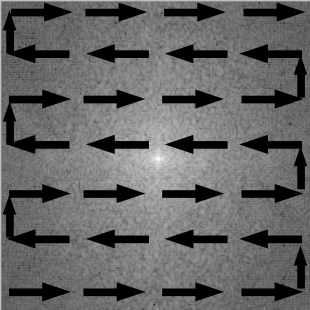
\includegraphics[width=2.5cm,height=2.5cm]{include/grp1/example_mask_kspace_with_arrows}
			
		} & \subfloat[\textcolor{black}{\scriptsize{}fully sampled MRI}]{\centering{}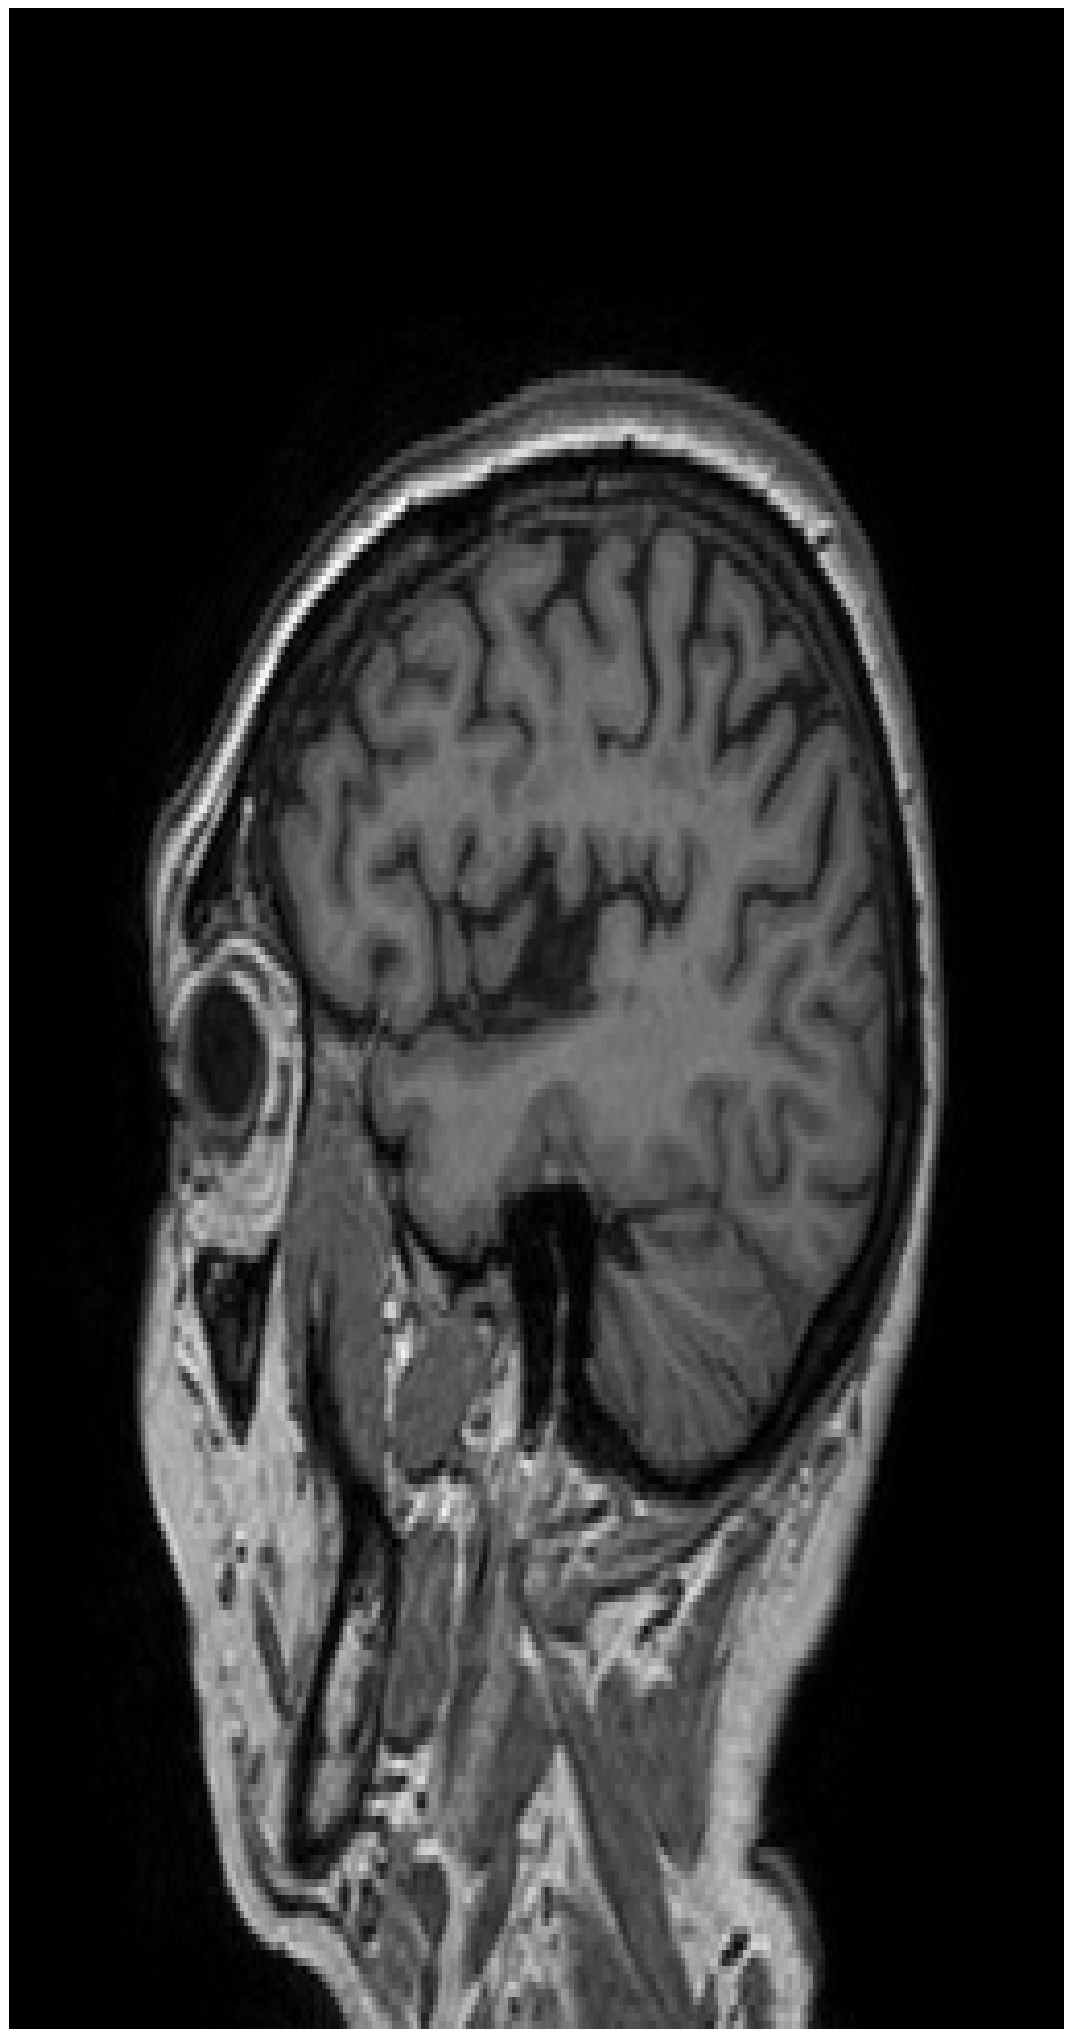
\includegraphics[width=2.5cm,height=2.5cm]{include/grp2/example_original.png}
		
		} & \subfloat[\textcolor{black}{\scriptsize{}sampling mask}]{\centering{}
\includegraphics[width=2.5cm,height=2.5cm]{include/grp2/example_samplingMask4.png}
	
		} & \subfloat[\textcolor{black}{\scriptsize{}Zero-filled}]{\centering{}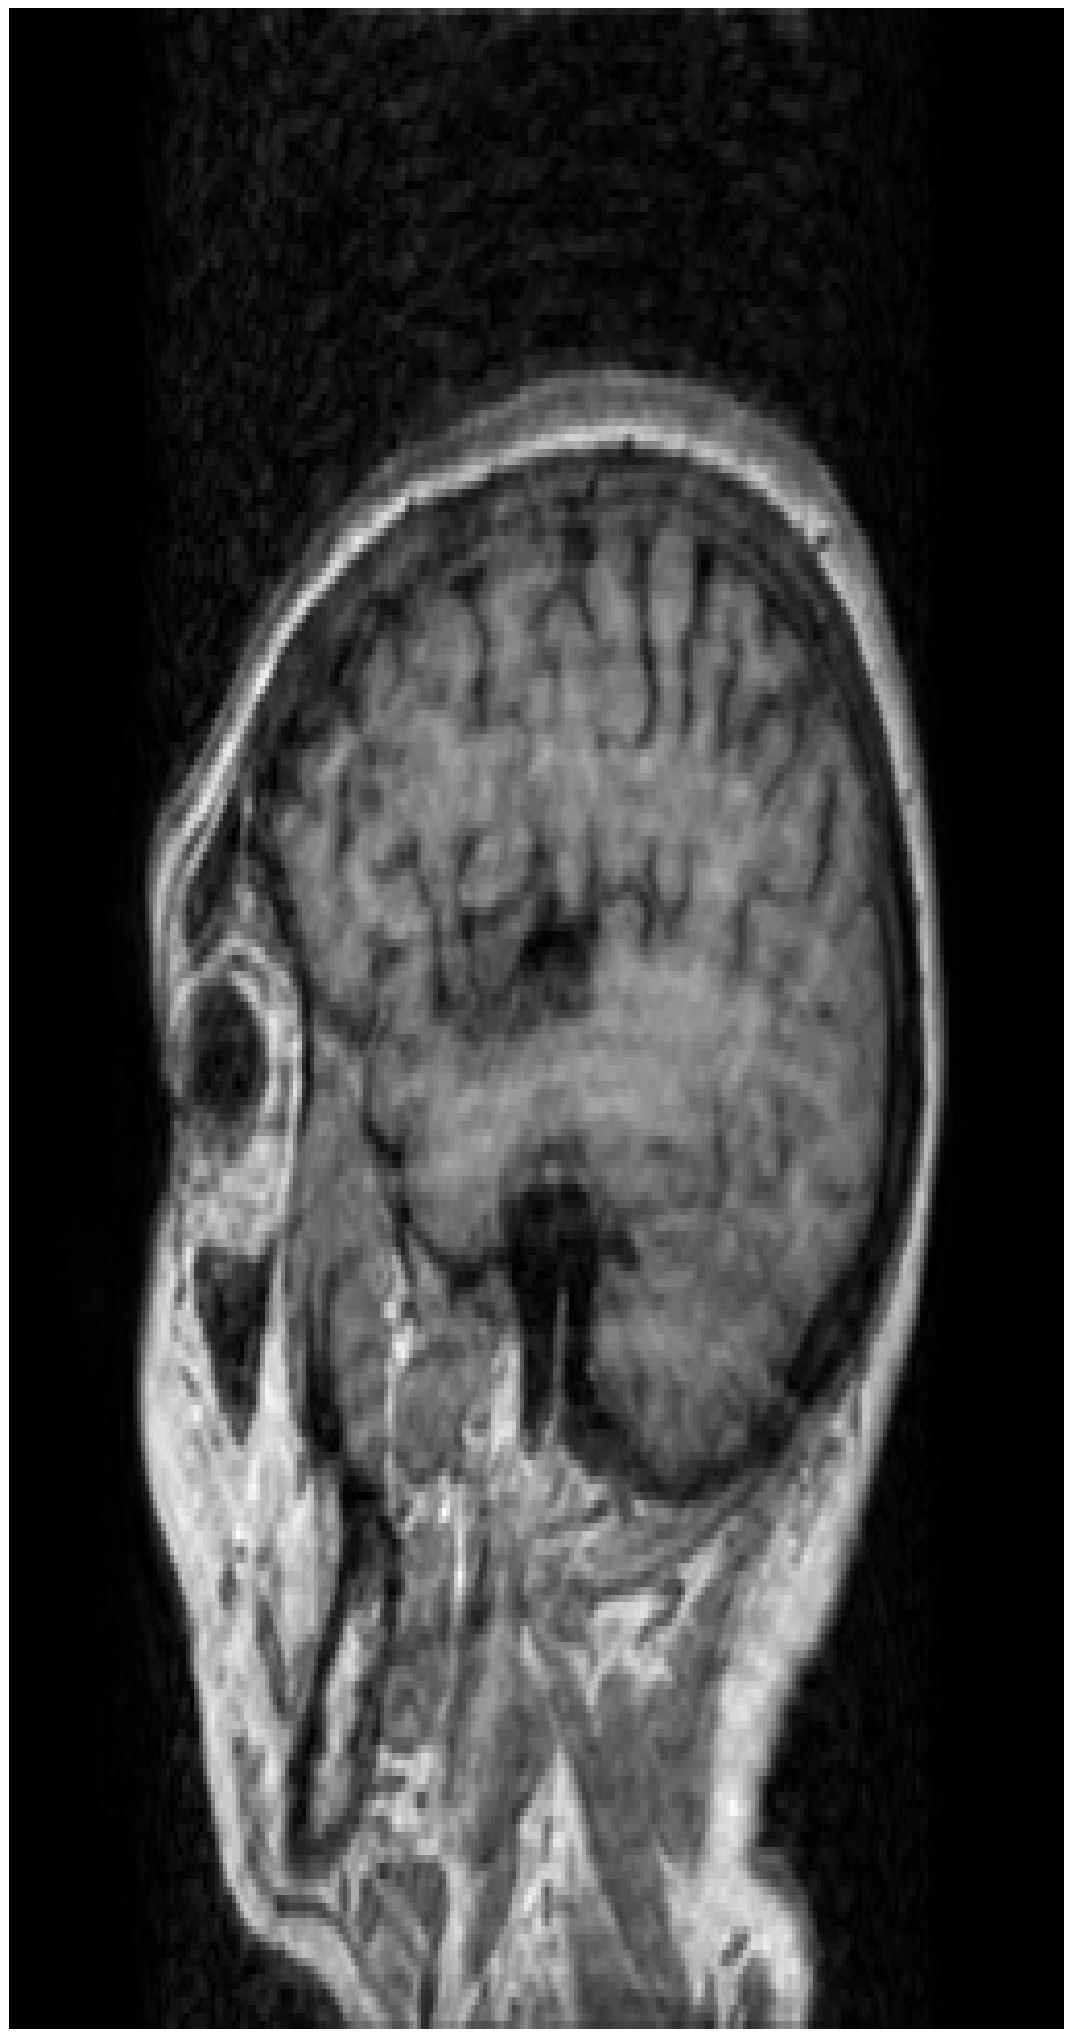
\includegraphics[width=2.5cm,height=2.5cm]{include/grp2/example_zeroPadding.png}
}\tabularnewline
\end{tabular}\caption{\textcolor{black}{\footnotesize{}{}Under-sampling artifacts: the
	arrows illustrate the sampling methodology}}
\label{fig:pair_of_k_space_mri} 
\end{figure}


\subsection{Objective}

Let $s_{p}=M_{p}\odot s_{0}$ denote the under-sampled k-space. Given
a sampling mask and a model $f$, defined by the set of parameters
$\Theta$, our goal is to estimate the missing k-space samples such
that: 
\begin{equation}
\Theta=\arg\min_{\Theta}L(F^{H}f\left(s_{p};\Theta\right),\boldsymbol{u})
\end{equation}
where $L\left(\cdot\right)$ is the loss function. While choosing
the loss to be L2 norm is reasonable for natural images, for the k-space,
which has different spatial features, this may not be enough. As mentioned
in \cite{pathak2016context}, L2 minimization provides a blurry solution.
Averaging the high frequency details in the k-space domain results
in very poor reconstruction. In order to address this problem, we
used the adversarial loss, based on GAN.

We trained our model using the adversarial strategy, as described
in \cite{goodfellow2014generative,radford2015unsupervised}. This
method is based on a generator $G$, which takes noise \textbf{$z$
}with uniform distribution \textbf{$p_{u}\left(z\right)$} as input
and generates samples from the data distribution. A discriminator
$D$ is trained to distinguish between ``real'' examples from the
data and generated (``fake'') examples from $G.$ During the training
process, we optimize $G$ to maximize the discriminator's probability
of error. Simultaneously, $D$ is getting better and provides more
accurate predictions.

Let $s_{0}$ denote a ``real'' k-space sample from the distribution
$p_{r}\left(s_{0}\right)$. The following optimization process can
be described by two-players min-max game:

\begin{equation}
\min_{G}\max_{D}\mathbb{E_{\mathrm{s_{0}\sim p_{r}\left(s_{0}\right)}}\mathrm{\log\left[D\left(x\right)\right]}}+\mathbb{E_{\mathrm{z\sim p_{u}\left(z\right)}}\mathrm{\log\left[1-D\left(G(z)\right)\right]}}
\end{equation}

In equilibrium, the generator $G$ is able to generate samples that
look like the real data. In our case, $G$ estimates the missing k-space
samples from a linear combination of the sampled data and a uniform
noise with distribution $p_{u}\left(z\right)$. An L2 fidelity constraint
is added to the adverbial loss of the generator, as follows:

\begin{equation}
\begin{aligned}L_{G}=\alpha\cdot E_{\mathrm{z\sim p_{u}\left(z\right)}}\mathrm{\log\left[1-D\left(F^{-1}\left(\hat{s}_{0}\right)\right)\right]}+\\
\beta\cdot||\left(1-M_{p}\right)\odot\left(\hat{s}_{0}-s_{0}\right)||_{2}^{2}
\end{aligned}
\end{equation}
where $\hat{s}_{0}$ is the estimated k-space and $\alpha=1,\,\beta=0.8$
are hyperparameters tuned by a cross-validation process. The discriminator's
input is the reconstructed MR image,\textbf{ }i.e.,\textbf{ }after
IFFT. By that, we are integrating the reconstruction phase in our
optimization.


\subsection{Network Architecture}

The generator input is a two-channel image representing the real and
the imaginary parts of the partially sampled k-space image, $s_{p}$.
Each missing sample is initialized by uniform i.i.d. noise. The pixel
$\left(i,j\right)$ in the generator input image is: 
\begin{equation}
G_{in}\left(i,j\right)=s_{p_{i,j}}+\left(1-M_{p}\right)_{i,j}z_{i,j}
\end{equation}

Due to the combination of the adversarial and the fidelity loss, $G$
produces reasonable k-space samples from a given samples and noise
distribution $p_{u}\left(z\right)$. In order to use the sampled data,
$s_{p}$, and estimate only the missing samples we used a residual
network \cite{he2016deep} as used in \cite{Oktay2016}, such that:
\begin{equation}
\hat{s}_{0}=s_{p}+\left(1-M_{p}\right)\odot G_{out}
\end{equation}
where $G_{out}$ is the generator output. Figure \ref{fig:system}
describes our framework:

\begin{figure}[H]
	\centering{}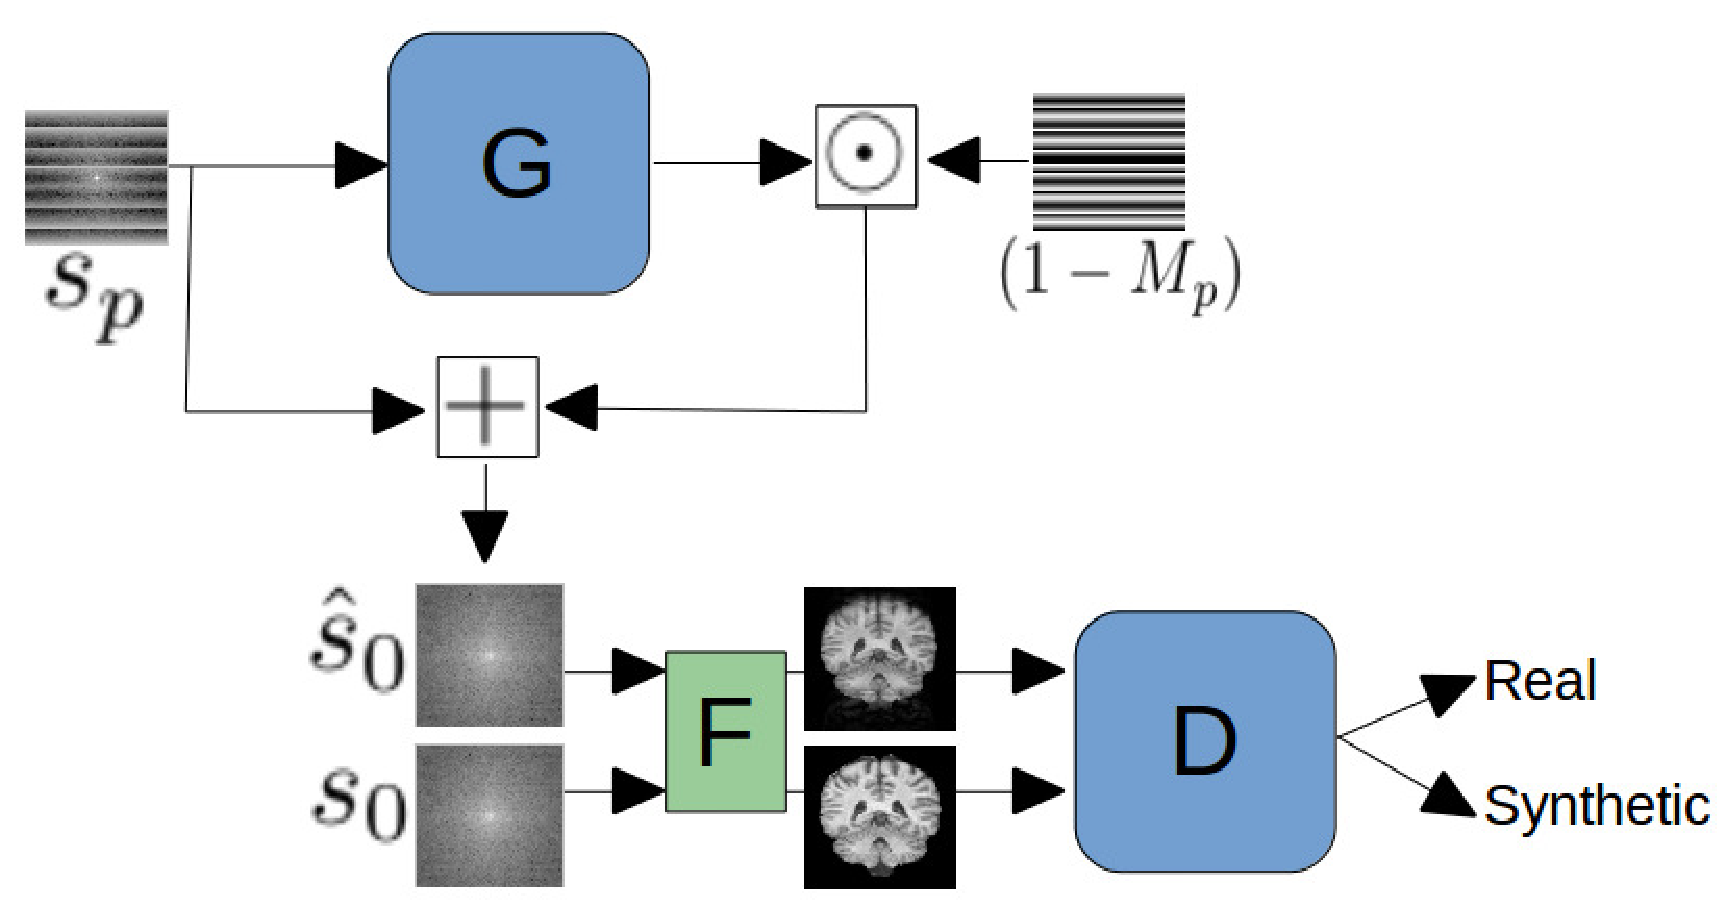
\includegraphics[width=7.8cm,height=4cm]{include/grp1/chart}\caption{\label{fig:system} \textcolor{black}{\footnotesize{}{}Framework
			architecture: $G$ and $D$ are the generator and discriminator networks,
			respectively. $F$ is a $2D$ IFFT operator.}}
\end{figure}


A common architecture is used for the discriminator, composed of convolutional
layers, batch normalization, and leaky-ReLU as suggested in \cite{radford2015unsupervised}.
For the generator, we compose a dedicated architecture based on multi-channel
input for representing the real and imaginary components. Both architectures
are shown in Figure \ref{fig:test}.\textbf{ }The training methodology
is doing $k_{g}$ generator update steps for each discriminator single
step.

\begin{figure*}
	\centering{}%
	\begin{tabular}{|c|}
		\hline 
		\subfloat[\textcolor{black}{\footnotesize{}Generator}]{\centering{}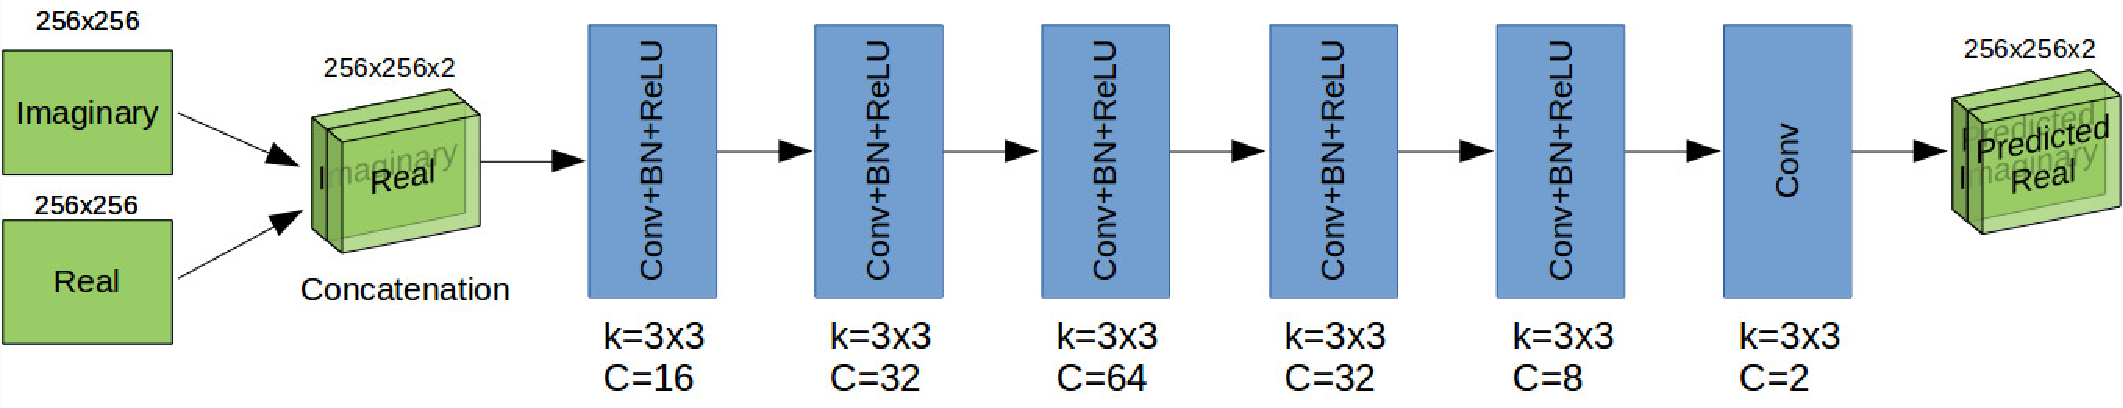
\includegraphics[width=12cm,height=2cm]{include/grp1/arch_generator} 
			
		}\tabularnewline
		\hline 
		\hline 
		\subfloat[\textcolor{black}{\footnotesize{}Discriminator}]{\centering{}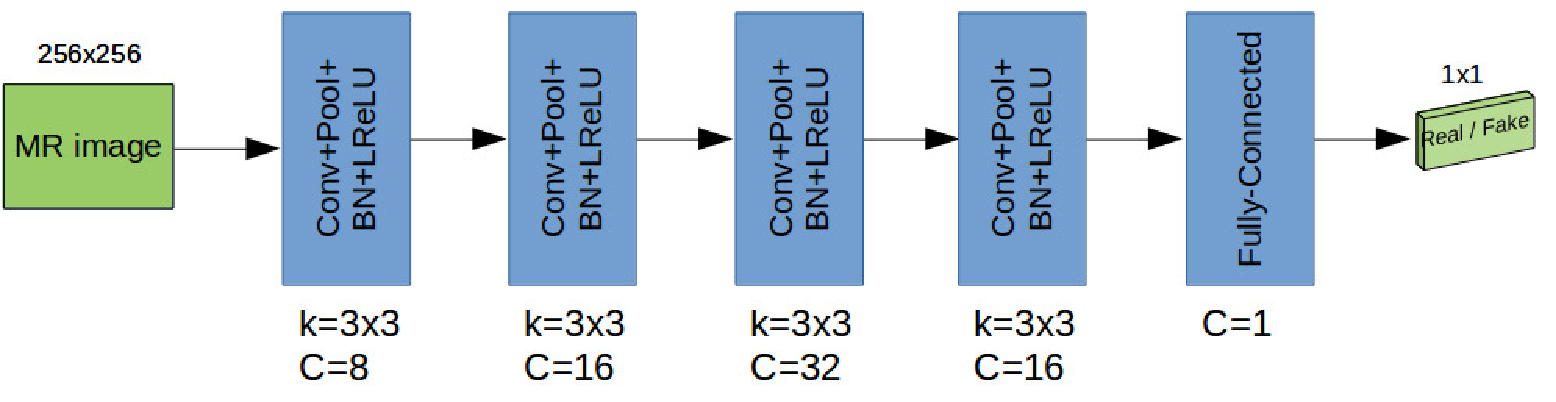
\includegraphics[width=9cm,height=2cm]{include/grp1/arch_discriminator} 
			
		}\tabularnewline
		\hline 
	\end{tabular}\caption{\textcolor{black}{\footnotesize{}{}Networks architecture. The generator
		input is a two-channel signal, real and imaginary. For each layer,
		$k$ is the kernel size and $C$ is the number of output channels.}}
\label{fig:test} 
\end{figure*}


%--------------------- Experiments --------------------%
\section{Experiments}

The training data consists of 500 $3D$ brain MRI (T1) scans of different patients from the IXI dataset\footnote{\url{http://brain-development.org/ixi-dataset/}}. The data has been acquired by three MR machines, Philips 1.5T, 3T and GE 1.5. All images padded to resolution of $256\times256$ pixels.
From each $3D$ volume we extract 93 $2D$ saggital slices. We used $37.2k$ $(80\%)$ 2D slices for training and $9.2k$ $(20\%)$ for testing (100 $3D$ volumes).
In order to create k-space images for training, inverse orthonormal
2D FFT is applied to the fully-sampled MR images. We sample the k-space
using $2D$ Gaussian mask with sampling factor of 2.5, 4 and 6. Data augmentation
is created by random offsets of the proposed mask and image flipping.
This leads us to reconstruction of the MR image from 40\%, 25\% and 16.6\% (Figure~\ref{fig:sampling_masks}) of
the original k-space data.

The generator is composed of $5$ blocks of CONV-BatchNorm-ReLU, with output channels $16,32,64,32,8,$ respectively. The last layer is CONV with two outputs channels (for real and imaginary parts). The discriminator is composed of $4$ blocks of CONV-Pool-BatchNorm-LReLU with output channels $8,16,32,16$ and one fully-connected layer. All CONV layers kernel size is $3\times3$. All weights was initialized by Xavier \cite{glorot2010understanding}. We used RMSprop solver with fixed learning rate of $5\mathrm{e}{-6}$ and set $k_{d}$ to 1.

We compare the proposed method to reconstruction results obtained by using a conventional compressed sensing method CS-MRI \cite{lustig2007sparse} and Zero-filling. In addition, we optimized two networks: 1. CNN-L2 - a k-space generator (with same architecture as the proposed method) using only L2 loss. 2. IM-CNN-L2 - a network which performs on the image-space and optimized to remove the artifacts caused by under-sampling and zero padding. We used the U-net \cite{ronneberger2015u} architecture inspired by \cite{lee2017deep}. The same sampling masks was used for all cases.

A common metric used to quantify the reconstructed image quality is the PSNR. In order to provide a reliable and robust evaluation of the reconstruction quality, which will be used for medical diagnostic, we suggest the following test: PSNR, brain's shape measure and tissue segmentation.

\begin{figure}[H]
	\centering
	\begin{tabular}{ccc}
		\subfloat[Factor 2.5 (40\%)]{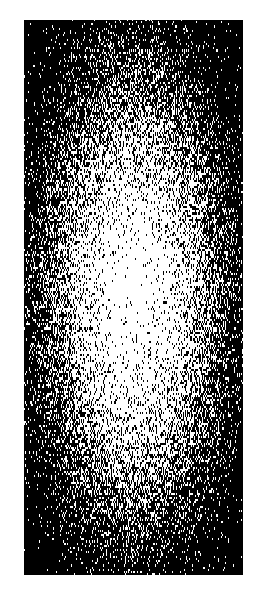
\includegraphics[width=3cm, height=3cm]{include/grp2/mask2}}
		& 
		\subfloat[Factor 4 (25\%)]{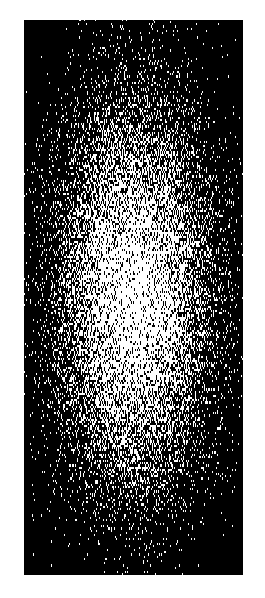
\includegraphics[width=3cm, height=3cm]{include/grp2/mask4}}
		&
		\subfloat[Factor 6 (16.66\%)]{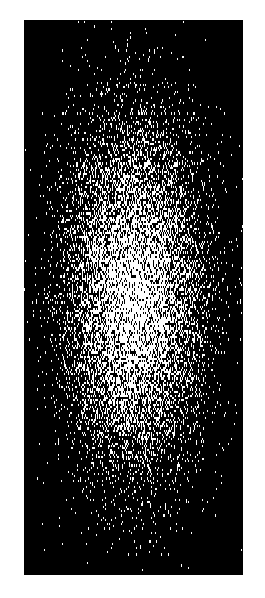
\includegraphics[width=3cm, height=3cm]{include/grp2/mask6}}
		\tabularnewline
		
	\end{tabular}\caption{$2D$ Gaussian sampling masks}
	\label{fig:sampling_masks}
\end{figure}

\subsection{Peak signal-to-noise ratio (PSNR)}
PSNR measures the Mean Squared Error (MSE) between the fully-sampled MR image and the reconstructed image. Therefore, this measure is not a sufficient metric for edges and general shape. For example, a model can provides a good reconstruction in the sense of PSNR but with blurry edges, which results in a poor performance of algorithms that use them, for example segmentation.
However, PSNR is still a good indication for the image quality, especially if an expert should view it.
Quantitative evaluation is presented in~Table~\ref{tbl:PSNR_NO_MASK} and a graphical visualization in ~Figure~\ref{fig:error_psnr_errorbar}. The PSNR calculated on the whole image without masking. Note that the proposed method outperforms the other.

%\begin{table}[H]
%	\centering{}
%\begin{tabular}{|c||c|c||c|c||c|c|}
%	\hline 
%	\textbf{PSNR} & \multicolumn{2}{c||}{Factor 2.5} & \multicolumn{2}{c||}{Factor 4} & \multicolumn{2}{c|}{Factor 6}\tabularnewline \cline{2-7}
%
%	\textbf{Method}     &Mean   &std    &Mean   &std     &Mean   &std \tabularnewline \hline 	
%	Zero-filled         &32.044 &2.616  &26.447 &1.997   &16.470 &2.181\tabularnewline
%	CS-MRI              &39.053 &2.479  &33.273 &2.452   &26.951 &3.380\tabularnewline
%	CNN-L2              &38.978 &2.454  &33.405 &2.232   &31.010 &2.299\tabularnewline
%	\textbf{Proposed}   &39.802 &2.489  &34.595 &2.519   &31.555 &2.487\tabularnewline
%		\hline 
%	\end{tabular}\caption{\textcolor{black}{\footnotesize{}{}Error in PSNR, without masking}{\footnotesize{}\label{tbl:PSNR_NO_MASK}}}
%\end{table}


\begin{table}[H]
	\centering{}
	\begin{tabular}{|c||c||c||c|}
		\hline 
		\textbf{PSNR} & \multicolumn{1}{c||}{\multirow{2}{*}{Factor 2.5}} & \multicolumn{1}{c||}{\multirow{2}{*}{Factor 4}} & \multicolumn{1}{c|}{\multirow{2}{*}{Factor 6}} \tabularnewline
		\textbf{Method} & \multicolumn{1}{c||}{} & \multicolumn{1}{c||}{} & \multicolumn{1}{c|}{} \tabularnewline \cline{1-4}
		
		Zero-filled         &32.044~$\pm$~2.616  &26.447~$\pm$~1.997   &16.470~$\pm$~2.181\tabularnewline
		CS-MRI              &39.053~$\pm$~2.479  &33.273~$\pm$~2.452   &26.951~$\pm$~3.380\tabularnewline
		IM-CNN-L2           &35.281~$\pm$~2.210  &31.577~$\pm$~2.109   &23.417~$\pm$~2.676\tabularnewline
		CNN-L2              &38.978~$\pm$~2.454  &33.405~$\pm$~2.232   &31.010~$\pm$~2.299\tabularnewline
		\textbf{Proposed}   &\textbf{39.802~$\pm$~2.489}  &\textbf{34.595~$\pm$~2.519}   &\textbf{31.555~$\pm$~2.487}\tabularnewline
		\hline 
	\end{tabular}\caption{\textcolor{black}{\footnotesize{}{}Error in PSNR, without masking}{\footnotesize{}\label{tbl:PSNR_NO_MASK}}}
\end{table}



\begin{figure}[H]
\centering
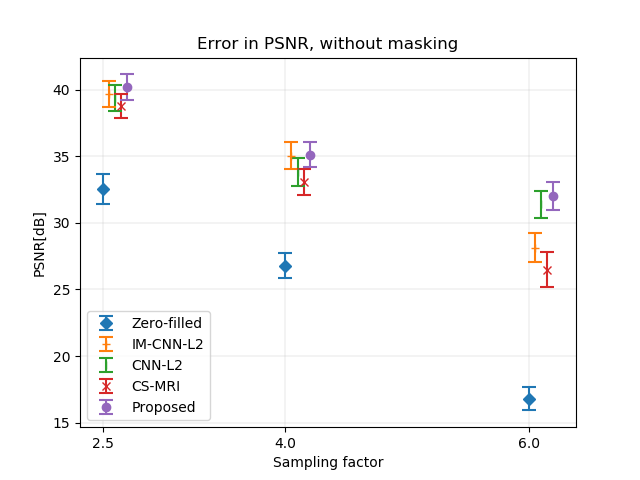
\includegraphics[width=0.7\linewidth]{include/grp2/error_psnr_errorbar}
\caption{PSNR without masking error-bar}
\end{figure}\label{fig:error_psnr_errorbar}

An extended validation of our model done by calculating the PSNR measure on different brain tissues. We applied an image segmentation algorithm, FAST \cite{zhang2001segmentation}, on the original fully-sampled MR image and then use it for calculating the masked-PSNR on gray matters, white matters and the Cerebrospinal Fluid (CSF). results are presented in~Table~\ref{tbl:PSNR_WITH_MASK}.


%\begin{table}[H]
%	\centering
%\begin{tabular}{|c||c|c|c||c|c|c||c|c|c|}
%	\hline 
%	\textbf{PSNR} & \multicolumn{3}{c||}{Factor 2.5} & \multicolumn{3}{c||}{Factor 4} & \multicolumn{3}{c|}{Factor 6}\tabularnewline
%	\cline{2-10} 
%	 \textbf{Method}& White & Gray & CSF & White & Gray & CSF & White & Gray & CSF\tabularnewline
%	 \hline 
%	 Zero-filled & 41.494 & 36.736 & 38.546 & 37.279 & 34.379 & 36.369 & 24.887 & 24.987 & 29.337\tabularnewline
%	 \hline 
%	 CS-MRI & 44.374 & 40.042 & 40.744 & 41.655 & 37.247 & 39.119 & 35.595 & 33.111 & 36.648\tabularnewline
%	 \hline 
%	 CNN-L2 & 45.727 & 41.593 & 41.689 & 43.265 & 40.151 & 40.247 & 41.119 & 39.277 & 39.102\tabularnewline
%	 \hline 
%	 \textbf{Proposed} & 46.206 & 41.942 & 41.616 & 43.857 & 40.109 & 40.496 & 41.919 & 39.014 & 39.366\tabularnewline
%	 \hline 
%\end{tabular}
%\caption{\textcolor{black}{\footnotesize{}{}Error in PSNR, with masking}{\footnotesize{}\label{tbl:PSNR_WITH_MASK}}}
%\end{table}

\begin{table}[H]
	\centering
	\resizebox{\textwidth}{!}{%
		\scriptsize
		\setlength\tabcolsep{2pt}
	\begin{tabular}{|c||c|c|c||c|c|c||c|c|c|}
		\hline 
		\textbf{PSNR} & \multicolumn{3}{c||}{Factor 2.5} & \multicolumn{3}{c||}{Factor 4} & \multicolumn{3}{c|}{Factor 6}\tabularnewline
		\cline{2-10} 
		\textbf{Method}& White & Gray & CSF & White & Gray & CSF & White & Gray & CSF\tabularnewline
		\hline 
		Zero-filled & 41.494{\tiny $\pm$}3.48 & 36.736{\tiny $\pm$}3.32 & 38.546{\tiny $\pm$}2.45 & 37.279{\tiny $\pm$}2.18 & 34.379{\tiny $\pm$}2.52 & 36.369{\tiny $\pm$}1.87 & 24.887{\tiny $\pm$}1.62 & 24.987{\tiny $\pm$}1.91 & 29.337{\tiny $\pm$}2.08\tabularnewline
		\hline 
		CS-MRI & 44.374{\tiny $\pm$}4.20 & 40.042{\tiny $\pm$}3.84 & 40.744{\tiny $\pm$}3.16 & 41.655{\tiny $\pm$}3.12 & 37.247{\tiny $\pm$}2.99 & 39.119{\tiny $\pm$}2.43 & 35.595{\tiny $\pm$}3.15 & 33.111{\tiny $\pm$}2.91 & 36.648{\tiny $\pm$}2.26\tabularnewline
		\hline 
		CNN-L2 & 45.727{\tiny $\pm$}4.70 & 41.593{\tiny $\pm$}4.16 & 41.689{\tiny $\pm$}3.69 & 43.265{\tiny $\pm$}2.95 & 40.151{\tiny $\pm$}3.15 & 40.247{\tiny $\pm$}2.47 & 41.119{\tiny $\pm$}2.48 & 39.277{\tiny $\pm$}2.65 & 39.102{\tiny $\pm$}1.93\tabularnewline
		\hline 
		\textbf{Proposed} & \textbf{46.206{\tiny $\pm$}4.77} & \textbf{41.942{\tiny $\pm$}4.34} & \textbf{41.616{\tiny $\pm$}2.45} & \textbf{43.857{\tiny $\pm$}3.16} & \textbf{40.109{\tiny $\pm$}3.25} & \textbf{40.496{\tiny $\pm$}2.57} & \textbf{41.919{\tiny $\pm$}2.77} & \textbf{39.014{\tiny $\pm$}2.88} & \textbf{39.366{\tiny $\pm$}2.17}\tabularnewline
		\hline 
	\end{tabular}
	}
	\caption{\textcolor{black}{\footnotesize{}{}Error in PSNR, with masking}{\footnotesize{}\label{tbl:PSNR_WITH_MASK}}}
\end{table}


ONLY 2 DIGITS
\begin{table}[H]
	\centering
	\resizebox{\textwidth}{!}{%
		\scriptsize
		\setlength\tabcolsep{2pt}
		\begin{tabular}{|c||c|c|c||c|c|c||c|c|c|}
			\hline 
			\textbf{PSNR} & \multicolumn{3}{c||}{Factor 2.5} & \multicolumn{3}{c||}{Factor 4} & \multicolumn{3}{c|}{Factor 6}\tabularnewline
			\cline{2-10} 
			\textbf{Method}& White & Gray & CSF & White & Gray & CSF & White & Gray & CSF\tabularnewline
			\hline 
			Zero-filled & 41.49{\tiny $\pm$}3.48 & 36.73{\tiny $\pm$}3.32 & 38.54{\tiny $\pm$}2.45 & 37.27{\tiny $\pm$}2.18 & 34.37{\tiny $\pm$}2.52 & 36.36{\tiny $\pm$}1.87 & 24.88{\tiny $\pm$}1.62 & 24.98{\tiny $\pm$}1.91 & 29.33{\tiny $\pm$}2.08\tabularnewline
			\hline 
			CS-MRI & 44.37{\tiny $\pm$}4.20 & 40.04{\tiny $\pm$}3.84 & 40.74{\tiny $\pm$}3.16 & 41.65{\tiny $\pm$}3.12 & 37.24{\tiny $\pm$}2.99 & 39.11{\tiny $\pm$}2.43 & 35.59{\tiny $\pm$}3.15 & 33.11{\tiny $\pm$}2.91 & 36.64{\tiny $\pm$}2.26\tabularnewline
			\hline 
			CNN-L2 & 45.72{\tiny $\pm$}4.70 & 41.59{\tiny $\pm$}4.16 & 41.68{\tiny $\pm$}3.69 & 43.26{\tiny $\pm$}2.95 & 40.15{\tiny $\pm$}3.15 & 40.24{\tiny $\pm$}2.47 & 41.11{\tiny $\pm$}2.48 & 39.27{\tiny $\pm$}2.65 & 39.10{\tiny $\pm$}1.93\tabularnewline
			\hline 
			\textbf{Proposed} & \textbf{46.20{\tiny $\pm$}4.77} & \textbf{41.94{\tiny $\pm$}4.34} & \textbf{41.61{\tiny $\pm$}2.45} & \textbf{43.85{\tiny $\pm$}3.16} & \textbf{40.11{\tiny $\pm$}3.25} & \textbf{40.49{\tiny $\pm$}2.57} & \textbf{41.91{\tiny $\pm$}2.77} & \textbf{39.01{\tiny $\pm$}2.88} & \textbf{39.36{\tiny $\pm$}2.17}\tabularnewline
			\hline 
		\end{tabular}
	}
	\caption{\textcolor{black}{\footnotesize{}{}Error in PSNR, with masking}{\footnotesize{}\label{tbl:PSNR_WITH_MASK2}}}
\end{table}

%TODO:add after images
%Visual comparison is shown in Figure~\ref{fig:results}. MRIs reconstructed by using the suggested adversarial loss have stronger contrast and no significant aliasing or artifacts.

\begin{figure}[H]
	\begin{raggedright}
		\begin{tabular}{>{\centering}b{0.2cm}lcccc}
			& \multicolumn{1}{c}{\footnotesize Original} & {\footnotesize Zero-filled} & {\footnotesize CS-MRI} & {\footnotesize CNN-L2} & {\footnotesize Proposed}\tabularnewline
			\multirow{1}{0.2cm}[2cm]{\begin{turn}{90} {\footnotesize Reconstructed} \end{turn}} &
			 
			 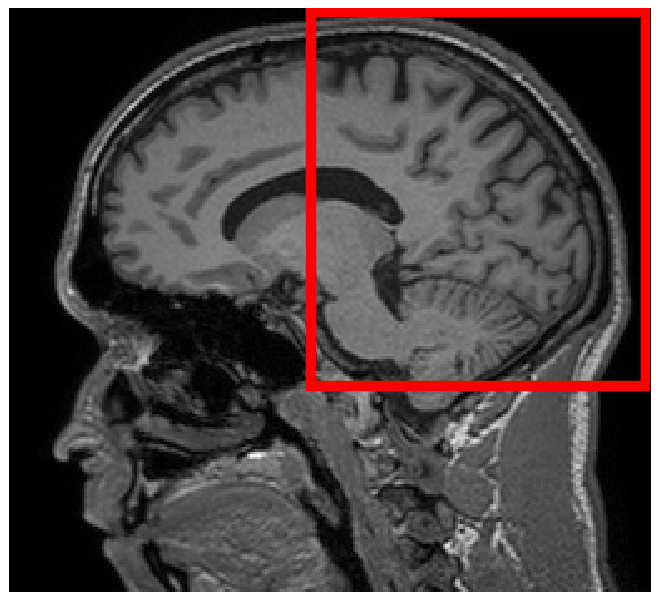
\includegraphics[width=2.5cm]{include/grp2/factor6/022-Guys-0701-T1/022-Guys-0701-T1_images__50} &
			 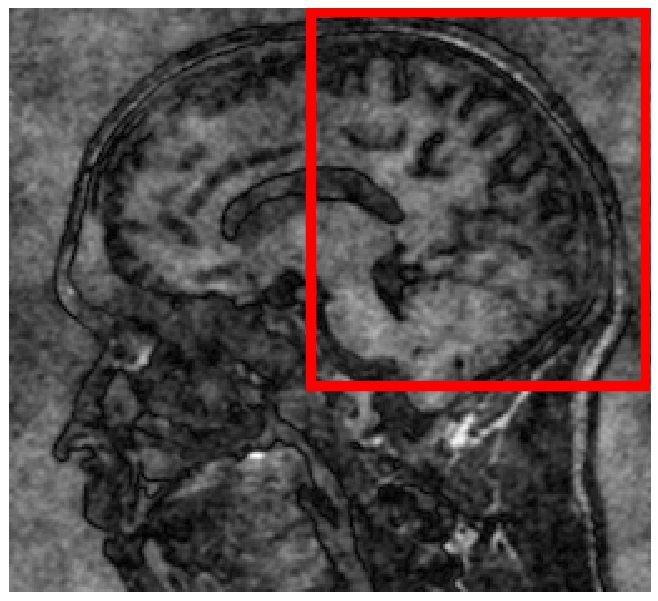
\includegraphics[width=2.5cm]{include/grp2/factor6/022-Guys-0701-T1/022-Guys-0701-T1_images__zeroPadding_50} & 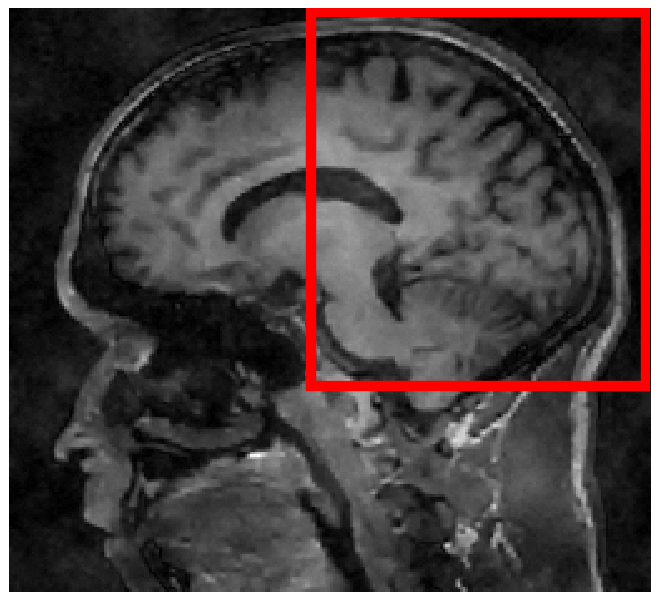
\includegraphics[width=2.5cm]{include/grp2/factor6/022-Guys-0701-T1/022-Guys-0701-T1_images__CS_50} & 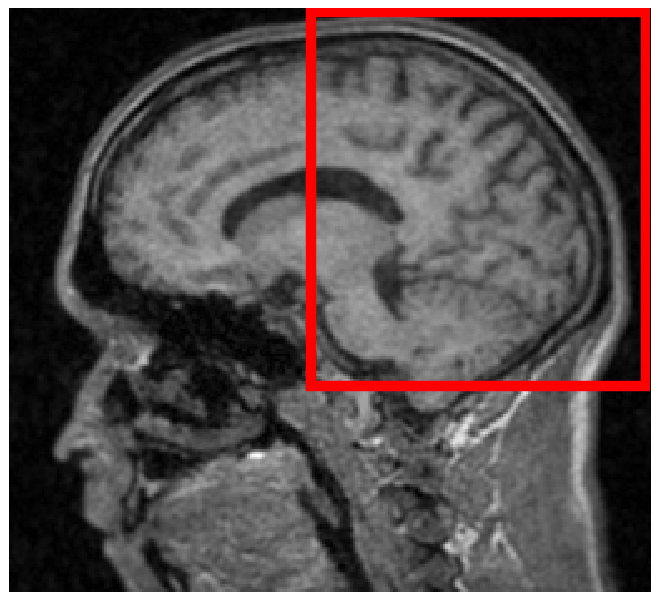
\includegraphics[width=2.5cm]{include/grp2/factor6/022-Guys-0701-T1/022-Guys-0701-T1_images__CNNL2_50} & 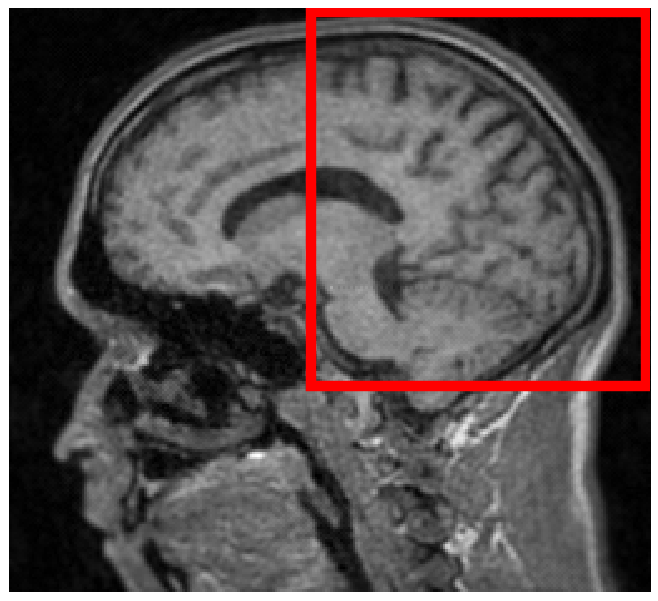
\includegraphics[width=2.5cm]{include/grp2/factor6/022-Guys-0701-T1/022-Guys-0701-T1_images__predict_50}
			 
			 \tabularnewline
			 
			 \multirow{1}{0.2cm}[2cm]{\begin{turn}{90} {\footnotesize Zoom in} \end{turn}} &
			
			 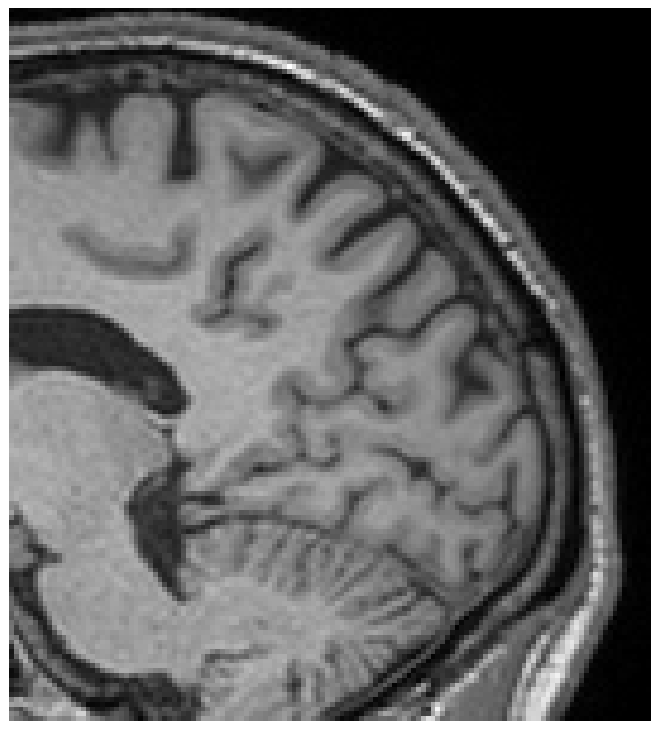
\includegraphics[width=2.5cm]{include/grp2/factor6/022-Guys-0701-T1/022-Guys-0701-T1_images__zoom_50} &
			 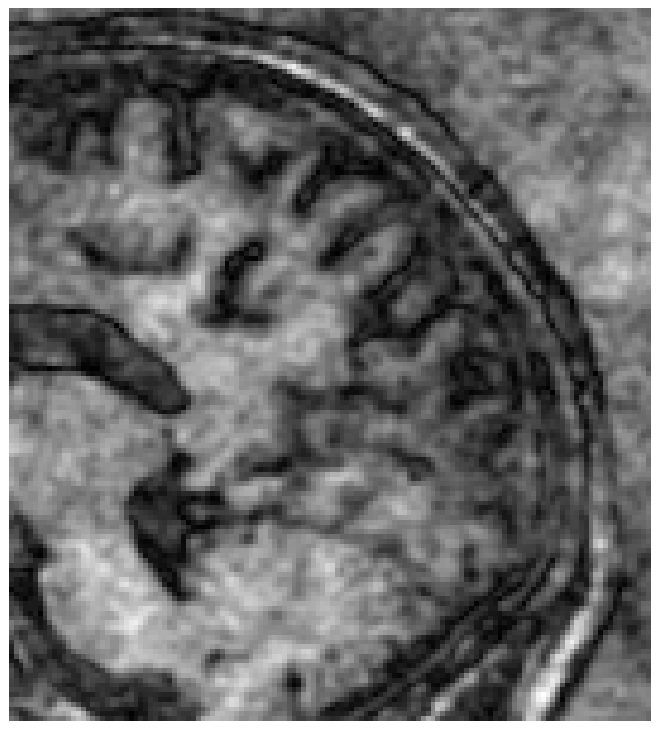
\includegraphics[width=2.5cm]{include/grp2/factor6/022-Guys-0701-T1/022-Guys-0701-T1_images__zeroPadding_zoom_50} & 
			 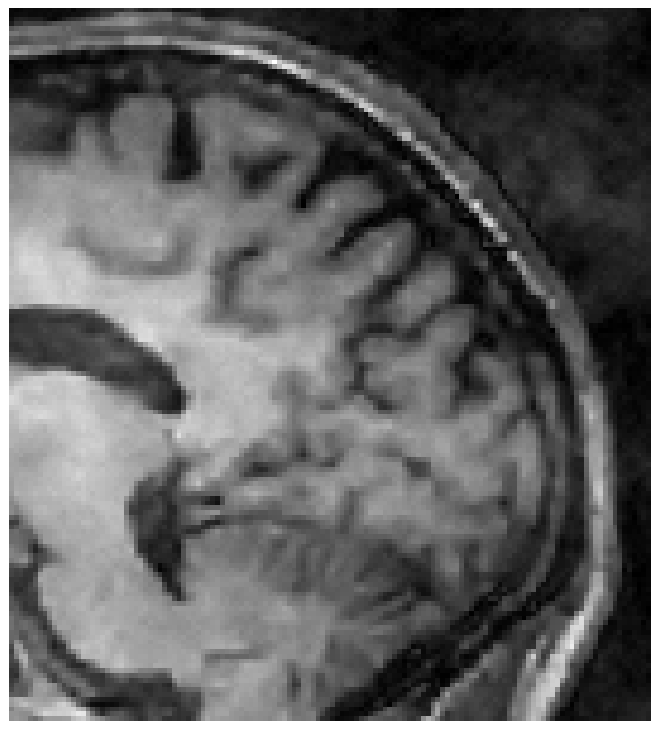
\includegraphics[width=2.5cm]{include/grp2/factor6/022-Guys-0701-T1/022-Guys-0701-T1_images__CS_zoom_50} & 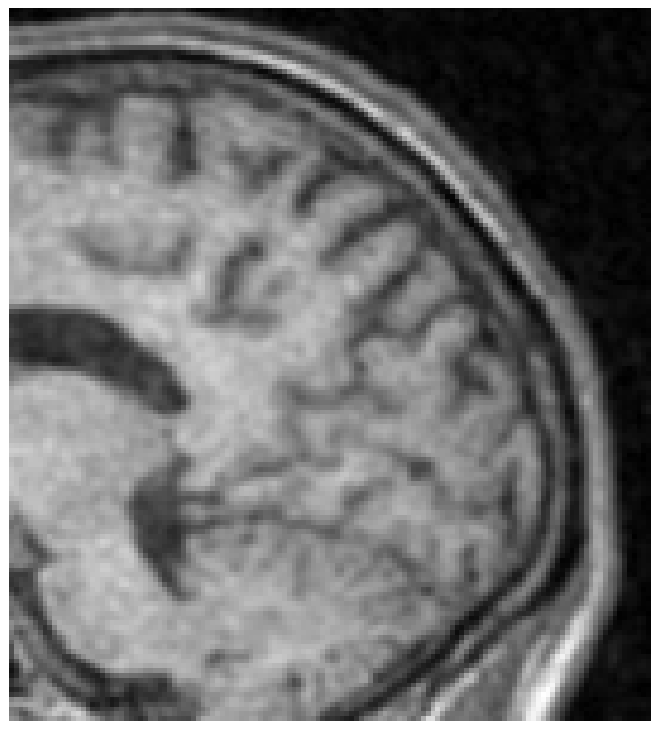
\includegraphics[width=2.5cm]{include/grp2/factor6/022-Guys-0701-T1/022-Guys-0701-T1_images__CNNL2_zoom_50} & 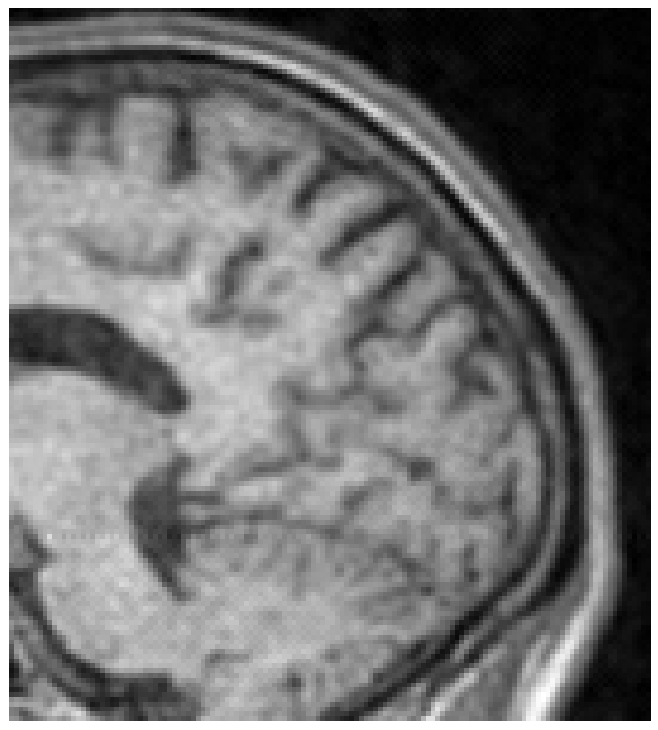
\includegraphics[width=2.5cm]{include/grp2/factor6/022-Guys-0701-T1/022-Guys-0701-T1_images__predict_zoom_50}
			 
			 \tabularnewline
			 
			\multirow{2}{0.2cm}[2cm]{\begin{turn}{90} {\footnotesize Brain} \end{turn}} & 
 			
 			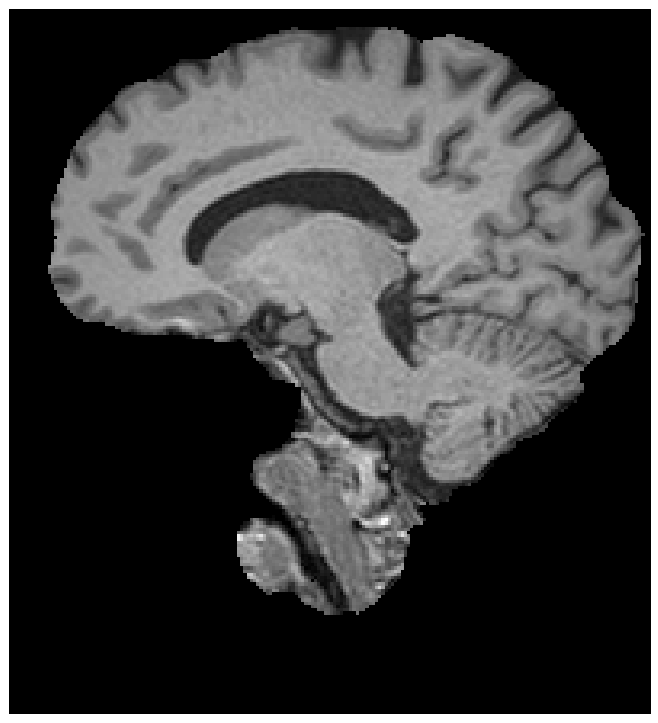
\includegraphics[width=2.5cm]{include/grp2/factor6/022-Guys-0701-T1/022-Guys-0701-T1_brains__50} &
			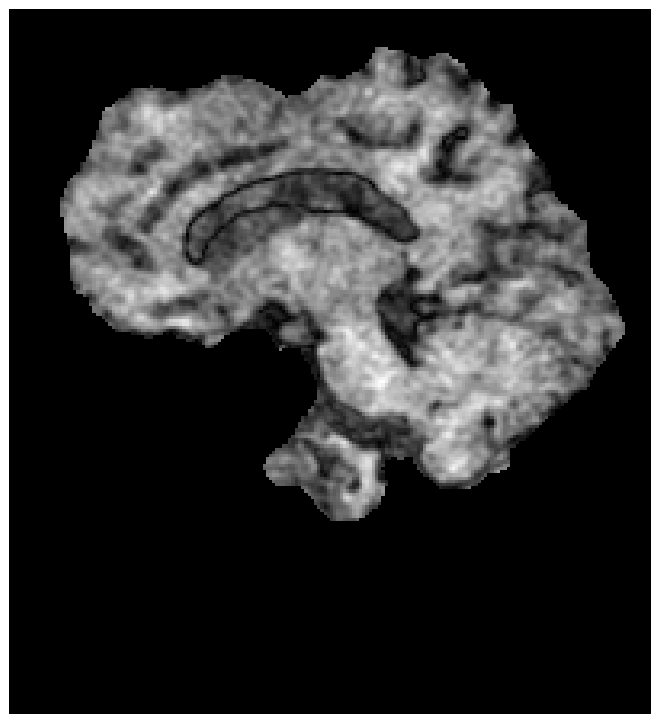
\includegraphics[width=2.5cm]{include/grp2/factor6/022-Guys-0701-T1/022-Guys-0701-T1_brains__zeroPadding_50} & 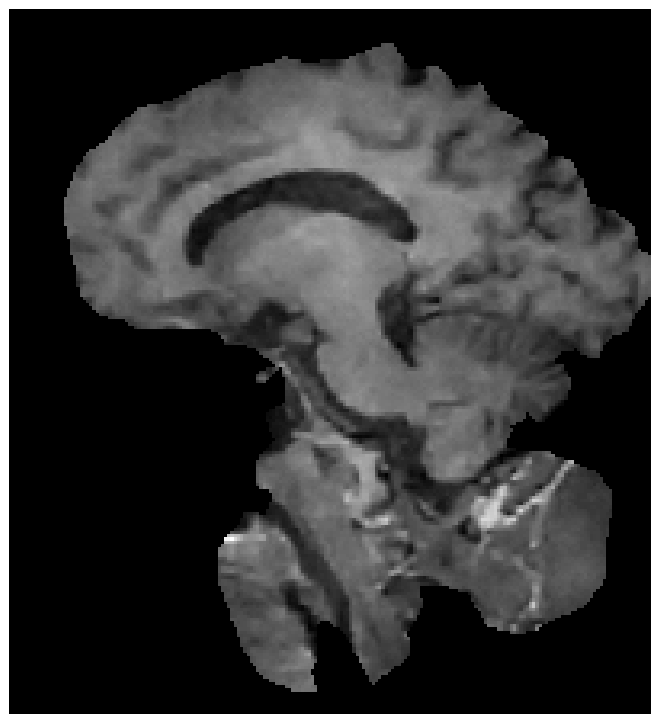
\includegraphics[width=2.5cm]{include/grp2/factor6/022-Guys-0701-T1/022-Guys-0701-T1_brains__CS_50} & 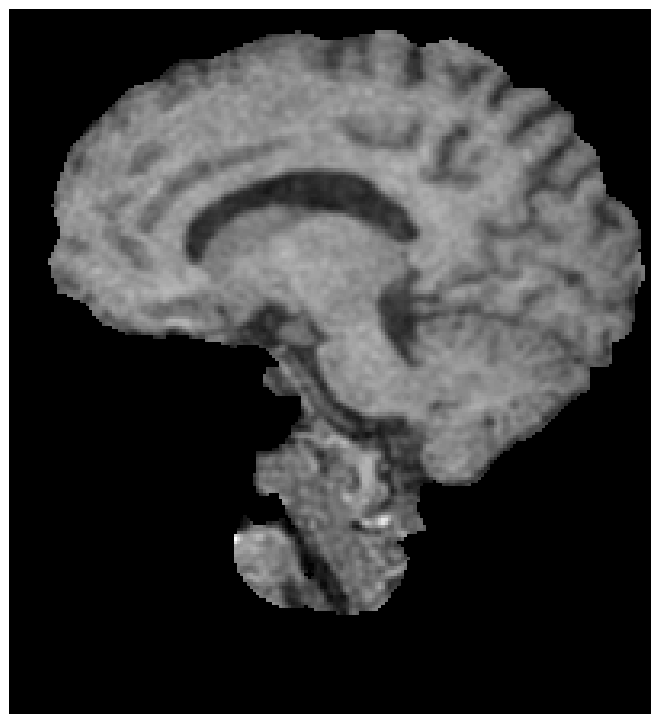
\includegraphics[width=2.5cm]{include/grp2/factor6/022-Guys-0701-T1/022-Guys-0701-T1_brains__CNNL2_50} & 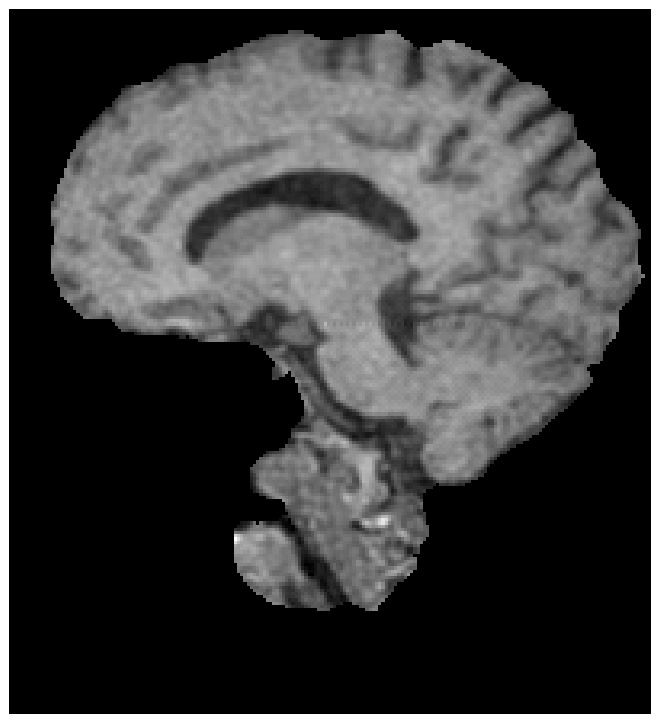
\includegraphics[width=2.5cm]{include/grp2/factor6/022-Guys-0701-T1/022-Guys-0701-T1_brains__predict_50}
			
			\tabularnewline
			
			\multirow{2}{0.2cm}[2cm]{\begin{turn}{90} {\footnotesize Segmentation} \end{turn}} & 
			
 			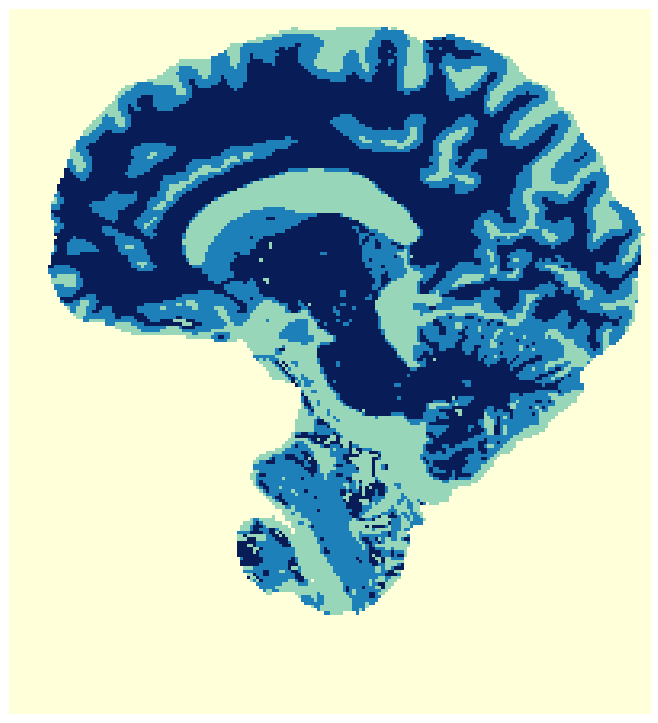
\includegraphics[width=2.5cm]{include/grp2/factor6/022-Guys-0701-T1/022-Guys-0701-T1_segs__50} &
 			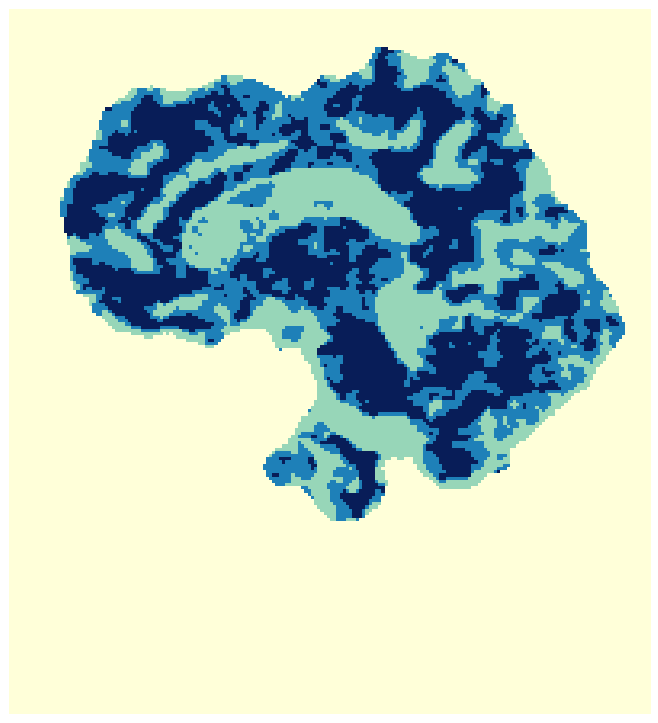
\includegraphics[width=2.5cm]{include/grp2/factor6/022-Guys-0701-T1/022-Guys-0701-T1_segs__zeroPadding_50} & 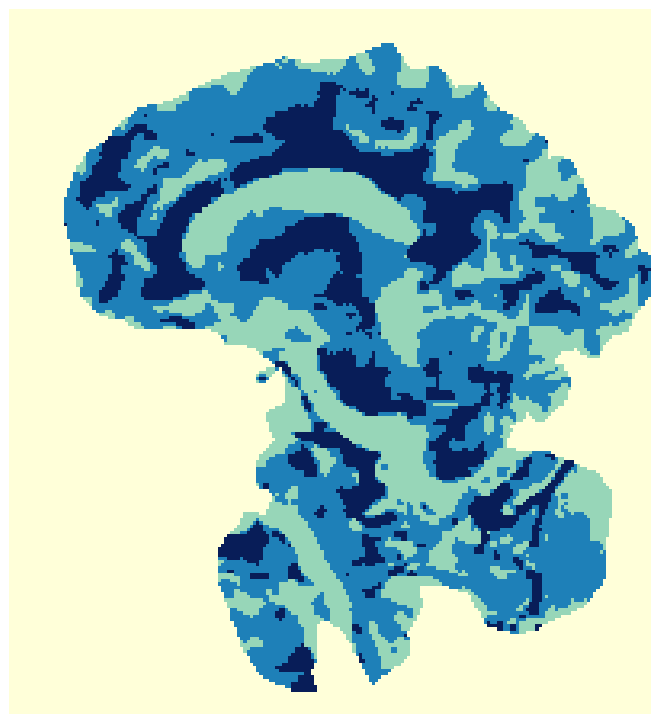
\includegraphics[width=2.5cm]{include/grp2/factor6/022-Guys-0701-T1/022-Guys-0701-T1_segs__CS_50} & 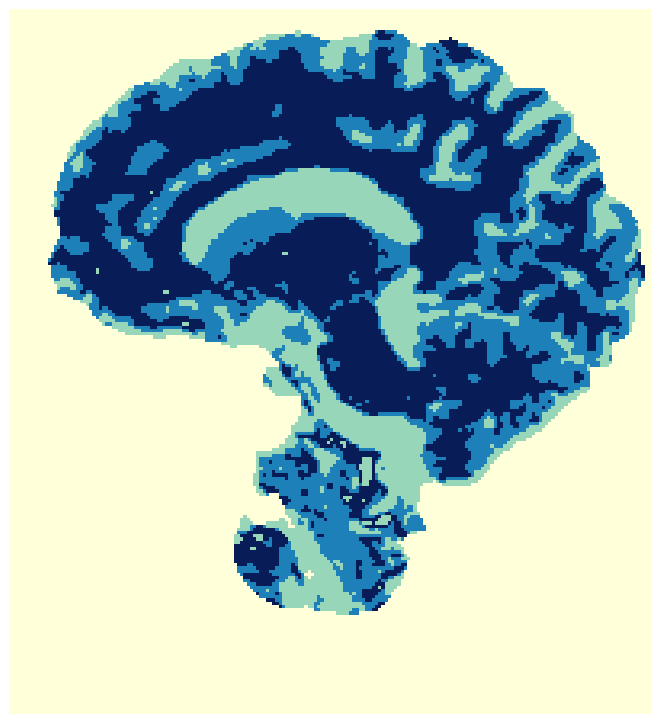
\includegraphics[width=2.5cm]{include/grp2/factor6/022-Guys-0701-T1/022-Guys-0701-T1_segs__CNNL2_50} & 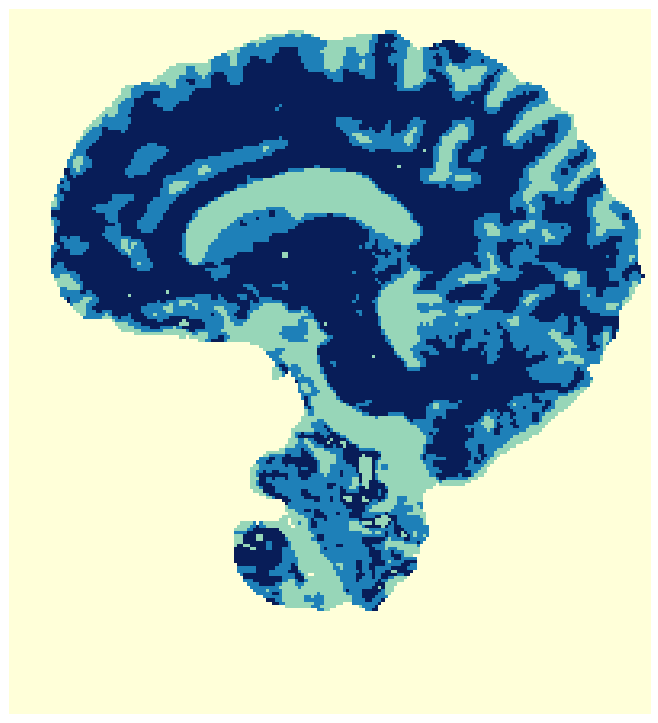
\includegraphics[width=2.5cm]{include/grp2/factor6/022-Guys-0701-T1/022-Guys-0701-T1_segs__predict_50}
			
			
		\end{tabular}
	\par\end{raggedright}
	\raggedright{}\caption{\textcolor{black}{\footnotesize{}Examples of reconstructed MR images from under-sampled k-space.}}
	\label{fig:example} 
\end{figure}


\subsection{Brain Extraction - Skull Stripping}
Brain extraction (Skull stripping) is a an algorithm that delineates the brain boundary (Figure~ \ref{fig:brain_extraction}). It is necessary for almost every brain analysis algorithm. In tissue segmentation for example, skull stripping is a pre-processing step which affects directly on the segments partition. We examine the different reconstruction methods by applying the Brain Extraction Tool (BET) \cite{smith2002fast} on each different MR reconstructed image. Then, we compared the skull stripping results to the fully-sampled result using the Modified Hausdorff Distance (MHD)~\cite{dubuisson1994modified}.

Let $C_1,C_2\in R^2$ denotes the brain contours extract from skull stripping algorithm on two different reconstruction methods respectively. MHD measures the distance between the contours such that:

\begin{equation}
\begin{array}{cc}
MHD(C_1,C_2) = \max \left\{\frac{1}{|C_1|} \sum_{\sigma_{1}\in C_1}^{}d(\sigma_1,C_2), ~ \frac{1}{|C_2|} \sum_{\sigma_{2}\in C_2}^{}d(\sigma_2,C_1)\right\} \\
d(\sigma_1,C_2) = \underset{\sigma_{2}\in C_{2}}{\min}||\sigma_1-\sigma_2|| \\
d(\sigma_2,C_1) = \underset{\sigma_{1}\in C_{1}}{\min}||\sigma_2-\sigma_1||
\end{array}
\end{equation}
where $\sigma_1,\sigma_2$ are points on the contours $C_1,C_2$ respectively (Figure~\ref{fig:brain_extraction}.c). MHD values for different sampling ratios are presented in~Table~\ref{tbl:MHD}.

\begin{table}[H]
	\centering{}
	\begin{tabular}{|c||c||c||c|}
		\hline 
		\textbf{MHD} & \multicolumn{1}{c||}{\multirow{2}{*}{Factor 2.5}} & \multicolumn{1}{c||}{\multirow{2}{*}{Factor 4}} & \multicolumn{1}{c|}{\multirow{2}{*}{Factor 6}} \tabularnewline
		\textbf{Method} & \multicolumn{1}{c||}{} & \multicolumn{1}{c||}{} & \multicolumn{1}{c|}{} \tabularnewline \cline{1-4}
				
		Zero-filled         &1.111~$\pm$~0.563  &2.617~$\pm$~1.214   &3.121~$\pm$~1.279\tabularnewline
		CS-MRI              &0.701~$\pm$~0.511  &1.447~$\pm$~1.027   &3.114~$\pm$~1.617\tabularnewline
		CNN-L2              &0.420~$\pm$~0.270  &0.715~$\pm$~0.561   &1.083~$\pm$~1.052\tabularnewline
		\textbf{Proposed}   &\textbf{0.391~$\pm$~0.250}  &\textbf{0.617~$\pm$~0.306}   &\textbf{1.050~$\pm$~1.033}\tabularnewline
		\hline 
	\end{tabular}\caption{\textcolor{black}{\footnotesize{}{}MHD - brain extraction}{\footnotesize{}\label{tbl:MHD}}}
\end{table}


\begin{figure}[H]
	\centering
	\begin{tabular}{ccc}
	\subfloat[MR image]{\includegraphics[width=3cm, height=3.5cm]{include/grp2/skull_stripping}} 
	& 
	\subfloat[Brain extraction]{\includegraphics[width=3cm, height=3.5cm]{include/grp2/skull_stripping_brain}}
	&
	\subfloat[Hausdorff distance]{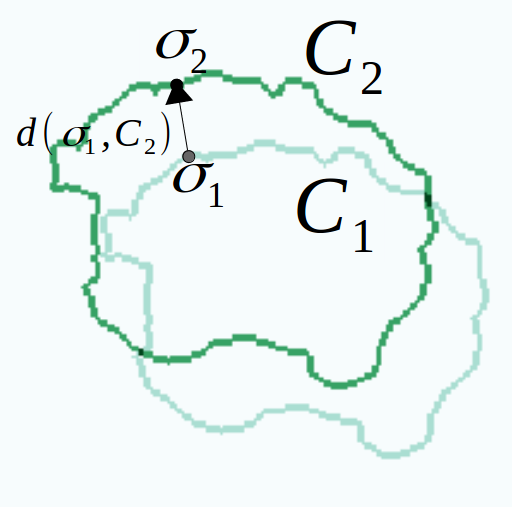
\includegraphics[width=3.5cm, height=3.5cm]{include/grp2/hausdorff}}
	\tabularnewline

	\end{tabular}\caption{Example of brain extraction}
	\label{fig:brain_extraction}
\end{figure}


\subsection{Brain Segmentation}
Brain segmentation is the task of partitioning the brain image (MRI in our case), into the following segments: background, white matter, gray matter and CSF. This process is of a great importance for brain MR image analysis, especially for therapy planning and also for clinical research. Sampling artifacts, results in poor signal to noise and blurry edges, may hurts the algorithm performance.
We suggest a way to evaluate and compare different MRI reconstruction methods based on segmentation results. We create a reference by extracting the brain (using BET \cite{smith2002fast}) from the original fully-sampled image and run a brain segmentation algorithm (FAST \cite{zhang2001segmentation}). Then, we did the same process for all the reconstruction methods and compared the segmentation results to the reference.

The measure used for segmentations comparison is the Dice score \cite{dice1945measures} between the original and the reconstructed image segments. Dice score is a measure of sets similarity which gets the values between 0 (no similarity) to 1.0 (max similarity). Denotes by $S_{i,j}$ the set of pixels in segment $j$ for method $i$, the Dice between two methods for this segment is:
\begin{equation}
\begin{array}{c}
DICE(S_{1,j},S_{2,j}) = \frac{2\cdot|S_{1,j} \cap S_{2,j}|} {|S_{1,j}| + |S_{2,j}|}
\end{array}
\end{equation}
Dice values for different sampling ratios are presented in~Table~\ref{tbl:DICE}. Our methods archive the best Dice score for all the brain tissues.

\begin{table}[H]
	\centering
	\resizebox{\textwidth}{!}{%
		\scriptsize
		\setlength\tabcolsep{2pt}
		\begin{tabular}{|c||c|c|c||c|c|c||c|c|c|}
			\hline 
			\textbf{DICE} & \multicolumn{3}{c||}{Factor 2.5} & \multicolumn{3}{c||}{Factor 4} & \multicolumn{3}{c|}{Factor 6}\tabularnewline
			\cline{2-10} 
			\textbf{Method}& White & Gray & CSF & White & Gray & CSF & White & Gray & CSF\tabularnewline
			\hline 
			Zero-filled & 0.882{\tiny $\pm$}0.08 & 0.826{\tiny $\pm$}0.05 & 0.796{\tiny $\pm$}0.05 & 0.718{\tiny $\pm$}0.10 & 0.644{\tiny $\pm$}0.05 & 0.627{\tiny $\pm$}0.05 & 0.599{\tiny $\pm$}0.12 & 0.466{\tiny $\pm$}0.07 & 0.050{\tiny $\pm$}0.06\tabularnewline
			\hline 
			CS-MRI & 0.942{\tiny $\pm$}0.05 & 0.910{\tiny $\pm$}0.03 & 0.868{\tiny $\pm$}0.03 & 0.871{\tiny $\pm$}0.10 & 0.805{\tiny $\pm$}0.08 & 0.770{\tiny $\pm$}0.05 & 0.708{\tiny $\pm$}0.14 & 0.639{\tiny $\pm$}0.08 & 0.621{\tiny $\pm$}0.07     \tabularnewline
			\hline 
			CNN-L2 & 0.948{\tiny $\pm$}0.02 & 0.919{\tiny $\pm$}0.02 & 0.891{\tiny $\pm$}0.02 & 0.888{\tiny $\pm$}0.06 & 0.836{\tiny $\pm$}0.04 & 0.813{\tiny $\pm$}0.03 & 0.836{\tiny $\pm$}0.09 & 0.770{\tiny $\pm$}0.06 & 0.747{\tiny $\pm$}0.06     \tabularnewline
			\hline
			
			\textbf{Proposed} & \textbf{0.954{\tiny $\pm$}0.01} & \textbf{0.928{\tiny $\pm$}0.02} & \textbf{0.900{\tiny $\pm$}0.002} & \textbf{0.903{\tiny $\pm$}0.06} & \textbf{0.858{\tiny $\pm$}0.04} & \textbf{0.833{\tiny $\pm$}0.03} & \textbf{0.851{\tiny $\pm$}0.09} & \textbf{0.789{\tiny $\pm$}0.06} & \textbf{0.767{\tiny $\pm$}0.06}     \tabularnewline
			\hline 
		\end{tabular}
	}
	
	\caption{\textcolor{black}{\footnotesize{}{}Segmentation Dice score for different sampling ratios}{\footnotesize{}\label{tbl:DICE}}}
	
\end{table}

%--------------------- CONCLUSIONS --------------------%
\section{Discussion}


We proposed a software-only framework, using GANs for accelerating MRI acquisition. Specifically, high-quality MRI reconstruction using only 40\%, 25\% and 16.6\% of the original k-space data is demonstrated. The key idea is based on utilizing an adversarial loss in addition to L2 loss. Extensive evaluation of the reconstruction quality was conducted in order to emphasize the advantage of proposed method.
Future work will concentrate on generation of MRI in the presence of pathologies.


%--------------------- Acknowledgment --------------------%
\subsection{Acknowledgment}
This research is partially supported by the Israel Science Foundation (T.R.R. 1638/16 ) and the IDF Medical Corps (T.R.R.)


\begin{figure}
	\begin{raggedright}
		
%		\hspace{-1.2cm}%
		\begin{tabular}{>{\centering}b{0.2cm}lcccc}
			& \multicolumn{1}{c}{{\footnotesize{}Original}} & {\footnotesize{}Zero-filled} & {\footnotesize{}CS-MRI} & {\footnotesize{}CNN-L2} & {\footnotesize{}Proposed}\tabularnewline
			\multirow{1}{0.2cm}[2cm]{\begin{turn}{90}
					{\footnotesize{}Reconstructed}
				\end{turn}} & 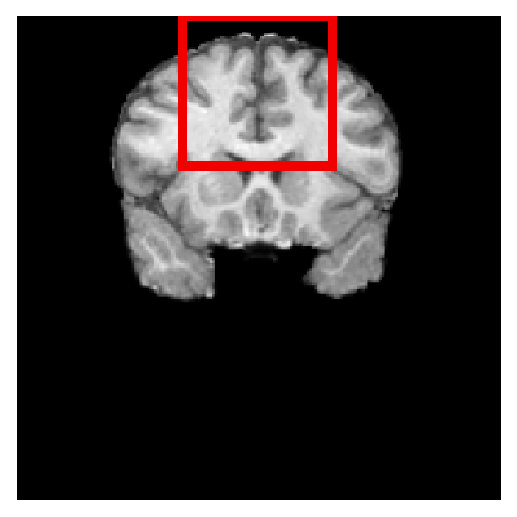
\includegraphics[width=2.5cm]{include/grp1/res1_org} & 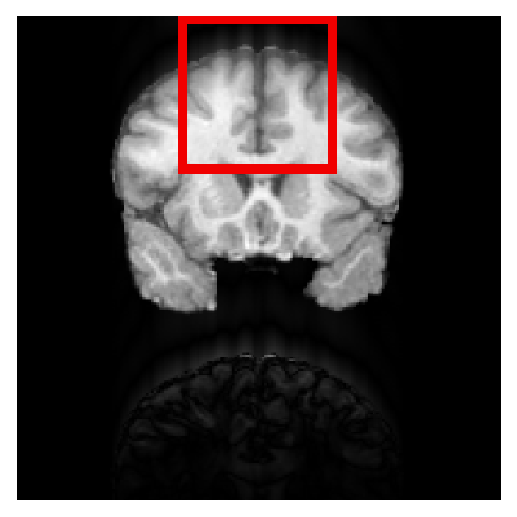
\includegraphics[width=2.5cm]{include/grp1/res1_zero} & 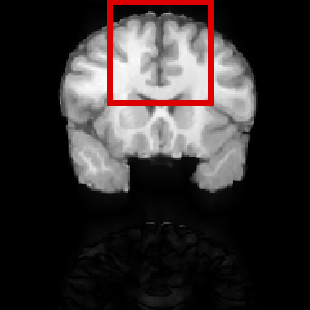
\includegraphics[width=2.5cm]{include/grp1/res1_cs_red} & 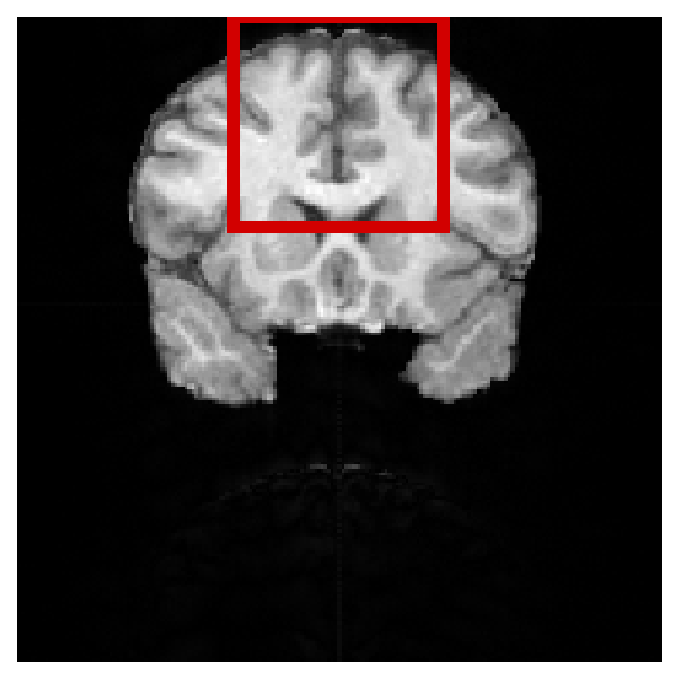
\includegraphics[width=2.5cm]{include/grp1/res1_L2_red} & 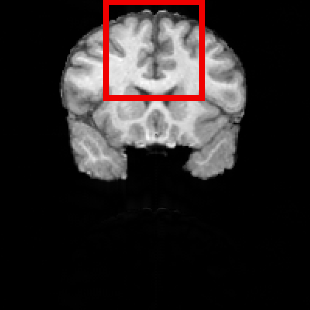
\includegraphics[width=2.5cm]{include/grp1/res1_our}\tabularnewline
				\multirow{1}{0.2cm}[2cm]{\begin{turn}{90}
						{\footnotesize{}Zoom in}
					\end{turn}} & 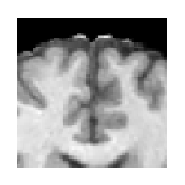
\includegraphics[width=2.5cm]{include/grp1/res1_org_zoom} & 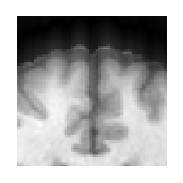
\includegraphics[width=2.5cm]{include/grp1/res1_zero_zoom} & 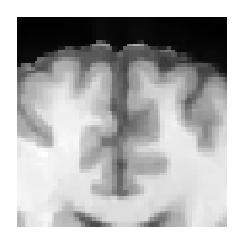
\includegraphics[width=2.5cm]{include/grp1/res1_cs_zoom} & 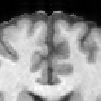
\includegraphics[width=2.5cm]{include/grp1/res1_L2_zoom} & 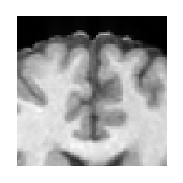
\includegraphics[width=2.5cm]{include/grp1/res1_our_zoom}\tabularnewline
					\multirow{1}{0.2cm}[2cm]{\begin{turn}{90}
							{\footnotesize{}Reconstructed}
						\end{turn}} & 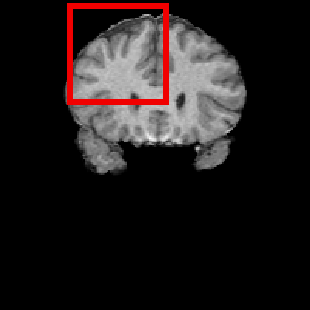
\includegraphics[width=2.5cm]{include/grp1/res7_org} & 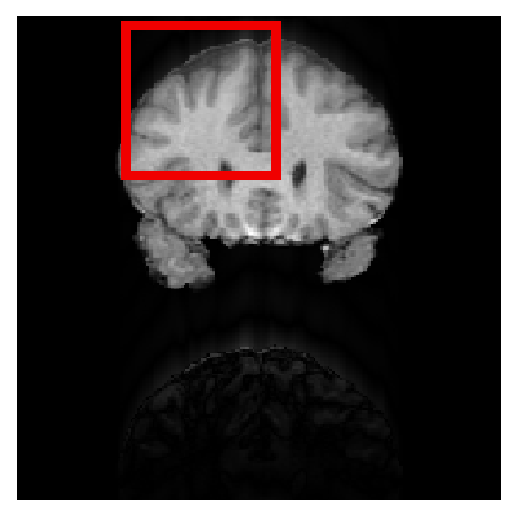
\includegraphics[width=2.5cm]{include/grp1/res7_zero} & 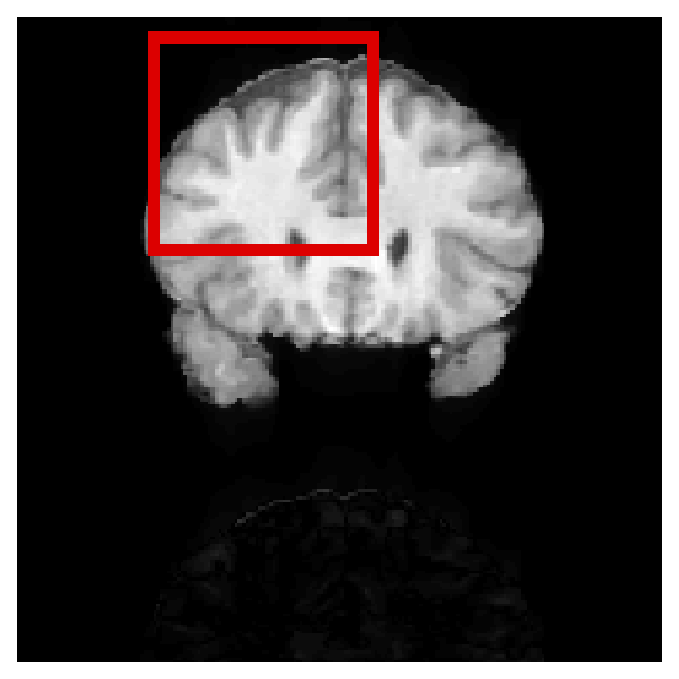
\includegraphics[width=2.5cm]{include/grp1/res7_cs_red} & 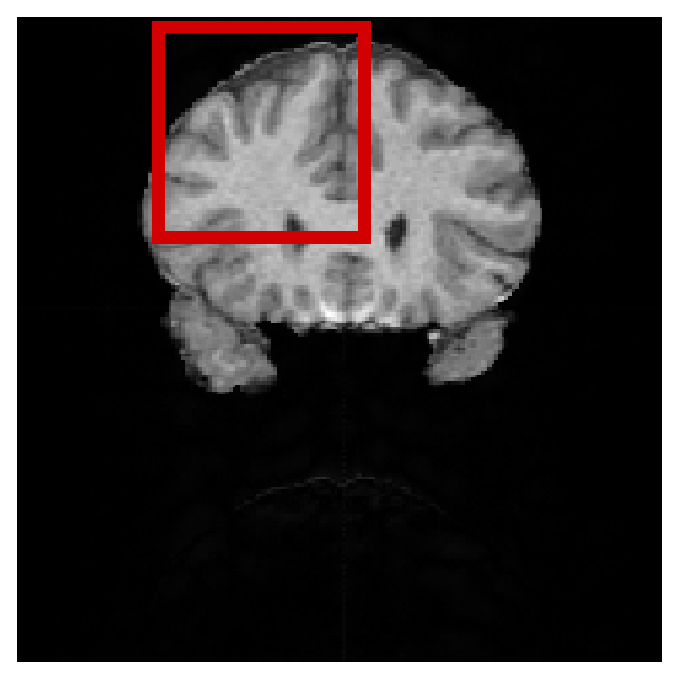
\includegraphics[width=2.5cm]{include/grp1/res7_L2_red} & 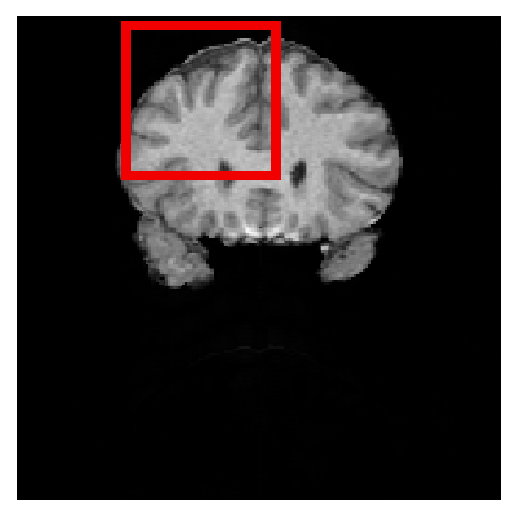
\includegraphics[width=2.5cm]{include/grp1/res7_our}\tabularnewline
						\multirow{1}{0.2cm}[2cm]{\begin{turn}{90}
								{\footnotesize{}Zoom in}
							\end{turn}} & 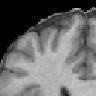
\includegraphics[width=2.5cm]{include/grp1/res7_org_zoom} & \includegraphics[width=2.5cm]{include/grp1/res7_zero_zoom} & \includegraphics[width=2.5cm]{include/grp1/res7_cs_zoom} & \includegraphics[width=2.5cm]{include/grp1/res7_L2_zoom} & \includegraphics[width=2.5cm]{include/grp1/res7_our_zoom}\tabularnewline
							\multirow{1}{0.2cm}[2cm]{\begin{turn}{90}
									{\footnotesize{}Reconstructed}
								\end{turn}} & \includegraphics[width=2.5cm]{include/grp1/res11_org} & \includegraphics[width=2.5cm]{include/grp1/res11_zero} & \includegraphics[width=2.5cm]{include/grp1/res11_cs_red} & \includegraphics[width=2.5cm]{include/grp1/res11_L2_red} & \includegraphics[width=2.5cm]{include/grp1/res11_our}\tabularnewline
								\multirow{1}{0.2cm}[2cm]{\begin{turn}{90}
										{\footnotesize{}Zoom in}
									\end{turn}} & \includegraphics[width=2.5cm]{include/grp1/res11_org_zoom} & \includegraphics[width=2.5cm]{include/grp1/res11_zero_zoom} & \includegraphics[width=2.5cm]{include/grp1/res11_cs_zoom} & \includegraphics[width=2.5cm]{include/grp1/res11_L2_zoom} & \includegraphics[width=2.5cm]{include/grp1/res11_our_zoom}\tabularnewline
								\end{tabular}
								\par\end{raggedright}
							\raggedright{}\caption{\textcolor{black}{\footnotesize{}Examples of reconstructed MR images
									from under-sampled k-space.}}
							\label{fig:results} 
						\end{figure}

\bibliography{paper}


\end{document}